%% LyX 2.3.4.2 created this file.  For more info, see http://www.lyx.org/.
%% Do not edit unless you really know what you are doing.
\documentclass[english,dvipsnames,aspectratio=169]{beamer}
% \documentclass[english,dvipsnames,aspectratio=169,handout]{beamer}
\usepackage{mathptmx}
\usepackage{eulervm}
\usepackage[T1]{fontenc}
\usepackage[latin9]{inputenc}
\usepackage{babel}
\usepackage{amstext}
\usepackage{amssymb}
\usepackage{graphicx}
\usepackage{ifthen}
\usepackage{xcolor}
\usepackage{xspace}
\usepackage{tikz}
\usetikzlibrary{tikzmark}
\usetikzlibrary{calc}
\usepackage{pgfplots}
%\pgfplotsset{compat=1.17}
\usepackage{booktabs}
\usepackage{xpatch}
\usepackage{multirow}
\usepackage{colortbl}
\usepackage{pgfpages}
\usepackage{bbm}

\xpatchcmd{\itemize}
  {\def\makelabel}
  {\ifnum\@itemdepth=1\relax
     \setlength\itemsep{2ex}% separation for first level
   \else
     \ifnum\@itemdepth=2\relax
       \setlength\itemsep{1ex}% separation for second level
     \else
       \ifnum\@itemdepth=3\relax
         \setlength\itemsep{0.5ex}% separation for third level
   \fi\fi\fi\def\makelabel
  }
 {}
 {}

\ifx\hypersetup\undefined
  \AtBeginDocument{%
    \hypersetup{unicode=true,pdfusetitle,
 bookmarks=true,bookmarksnumbered=false,bookmarksopen=false,
 breaklinks=false,pdfborder={0 0 0},pdfborderstyle={},backref=false,colorlinks=true,
 allcolors=NYUPurple,urlcolor=LightPurple}
  }
\else
  \hypersetup{unicode=true,pdfusetitle,
 bookmarks=true,bookmarksnumbered=false,bookmarksopen=false,
 breaklinks=false,pdfborder={0 0 0},pdfborderstyle={},backref=false,colorlinks=true,
 allcolors=NYUPurple,urlcolor=LightPurple}
\fi

\makeatletter

%%%%%%%%%%%%%%%%%%%%%%%%%%%%%% LyX specific LaTeX commands.
%% Because html converters don't know tabularnewline
\providecommand{\tabularnewline}{\\}

%%%%%%%%%%%%%%%%%%%%%%%%%%%%%% Textclass specific LaTeX commands.
% this default might be overridden by plain title style
\newcommand\makebeamertitle{\frame{\maketitle}}%
% (ERT) argument for the TOC
\AtBeginDocument{%
  \let\origtableofcontents=\tableofcontents
  \def\tableofcontents{\@ifnextchar[{\origtableofcontents}{\gobbletableofcontents}}
  \def\gobbletableofcontents#1{\origtableofcontents}
}

%%%%%%%%%%%%%%%%%%%%%%%%%%%%%% User specified LaTeX commands.
\usetheme{CambridgeUS} 
\beamertemplatenavigationsymbolsempty


% Set Color ==============================
\definecolor{NYUPurple}{RGB}{87,6,140}
\definecolor{LightPurple}{RGB}{165,11,255}


\setbeamercolor{title}{fg=NYUPurple}
\setbeamercolor{frametitle}{fg=NYUPurple}

\setbeamercolor{background canvas}{fg=NYUPurple, bg=white}
\setbeamercolor{background}{fg=black, bg=NYUPurple}

\setbeamercolor{palette primary}{fg=black, bg=gray!30!white}
\setbeamercolor{palette secondary}{fg=black, bg=gray!20!white}
\setbeamercolor{palette tertiary}{fg=gray!20!white, bg=NYUPurple}

\setbeamertemplate{headline}{}
\setbeamerfont{itemize/enumerate body}{}
\setbeamerfont{itemize/enumerate subbody}{size=\normalsize}

\setbeamercolor{parttitle}{fg=NYUPurple}
\setbeamercolor{sectiontitle}{fg=NYUPurple}
\setbeamercolor{sectionname}{fg=NYUPurple}
\setbeamercolor{section page}{fg=NYUPurple}
%\setbeamercolor{description item}{fg=NYUPurple}
%\setbeamercolor{block title}{fg=NYUPurple}

\setbeamertemplate{blocks}[rounded][shadow=false]
\setbeamercolor{block body}{bg=normal text.bg!90!NYUPurple}
\setbeamercolor{block title}{bg=NYUPurple!30, fg=NYUPurple}



\AtBeginSection[]{
  \begin{frame}
  \vfill
  \centering
\setbeamercolor{section title}{fg=NYUPurple}
 \begin{beamercolorbox}[sep=8pt,center,shadow=true,rounded=true]{title}
    \usebeamerfont{title}\usebeamercolor[fg]{title}\insertsectionhead\par%
  \end{beamercolorbox}
  \vfill
  \end{frame}
}

\makeatother

\setlength{\parskip}{\medskipamount} 

\input ../macros

\begin{document}
\input ../rosenberg-macros

%\setbeameroption{show notes on second screen}

\title[CSCI-GA 2565]{Clustering and Latent Variable Models}
\author[]{Mengye Ren
\\ \quad\\
\small (Slides credit to David Rosenberg, He He, et al.)}
% \author{He He \\
% Slides based on Lecture
% \href{https://github.com/davidrosenberg/mlcourse/blob/gh-pages/Lectures/13a.k-means.pdf}{13a} from David Rosenberg's course materials (\url{https://github.com/davidrosenberg/mlcourse})
% }
\date[]{Dec 3, 2024}
\institute[]{NYU}

\makebeamertitle
\mode<article>{Just in article version}

\begin{frame}{Lecture Slides}
\begin{center}

\includegraphics[width=0.4\textwidth]{figures/qr_12.png}
\end{center}
\end{frame}

\section{K-means Clustering}

\begin{frame}
{Unsupervised learning}
\begin{description}[<+->]
\item[Goal] Discover interesting \emph{structure} in the data.
\item[Formulation] Density estimation: $p(x;\theta)$ (often with \emph{latent} variables).
\item[Examples]
\begin{itemize}[<.->]
\item Discover \emph{clusters}: cluster data into groups.
\item Discover \emph{factors}: project high-dimensional data to a small number of ``meaningful'' dimensions, \ie dimensionality reduction.
\item Discover \emph{graph structures}: learn joint distribution of correlated variables, \ie graphical models.
\end{itemize}
\end{description}
\note[item]{Most of what we have learned so far belongs to supervised learning, where the core problem is to make predictions on unseen data given labeled training data. There is another important type of ML called unsupervised learning, where the main goal is to discover interesting patterns in the data.}
\note[item]{Unlike supervised learning, there is no obvious loss function since we don't know what patterns to look for. Instead, the problem is often formulated as density estimation where we aim to maximize the likelihood of the observed data.}
\note[item]{Clusters: group documents into different topics.}
\note[item]{Factors: variation among face images can be explained by a few factors such as illumination, pose, identity etc.}
\note[item]{Graph: phylogenetic tree of DNA evolution.}
\note[item]{We'll focus on clustering today.}
\end{frame}

\begin{frame}{Example: Old Faithful Geyser}
\begin{center}
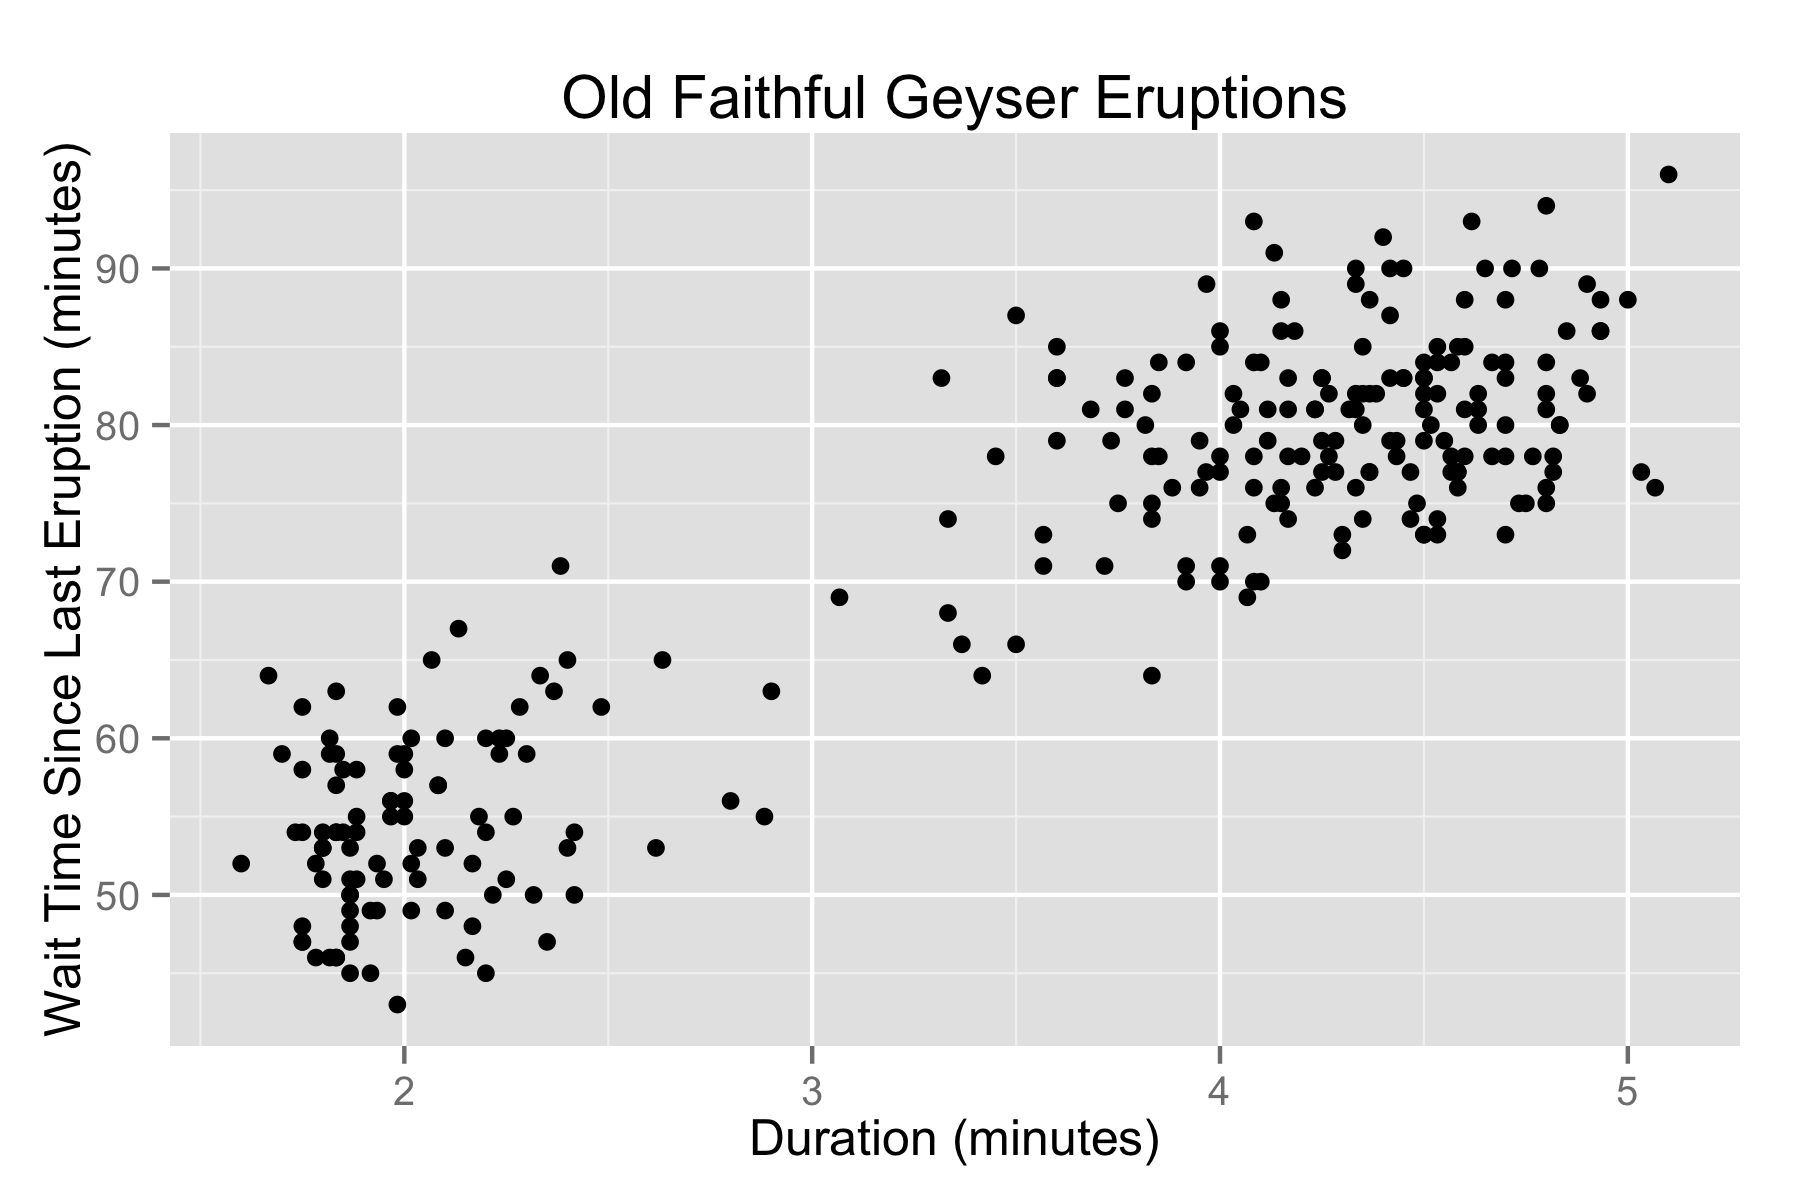
\includegraphics[height=0.6\textheight]{figures/oldfaithful}
\end{center}
\begin{itemize}
\item Looks like two clusters.
\item How to find these clusters algorithmically?
\end{itemize}
\note[item]{Let's consider a simple example. The old faithful geyser in Yellowstone has very predictable eruptions. It roughly erupts every 55 or 80 minutes. We can visualize this for 2D data, but how do we find these clusters more generally?}
\note[item]{One popular and simple algorithm is $k$-means. Let's go through the algorithm through this example.}
\end{frame}

\begin{frame}{$k$-Means: By Example}

\begin{itemize}
\item Standardize the data.
\item Choose two cluster centers.
\end{itemize}
\begin{center}
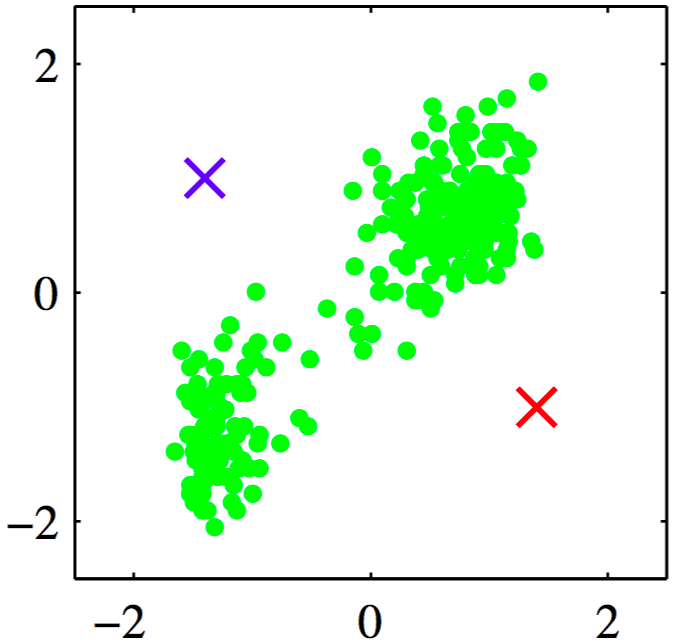
\includegraphics[height=0.55\textheight]{{figures/faithful-9.1a}}
\end{center}

\let\thefootnote\relax\footnotetext{\tiny{From Bishop's \emph{Pattern recognition and machine learning}, Figure 9.1(a).}}
\note[item]{We first standardize the data and choose two points randomly. They will be the cluster center.}
\end{frame}

\begin{frame}{$k$-means: by example}

\begin{itemize}
\item Assign each point to closest center.
\end{itemize}
\begin{center}
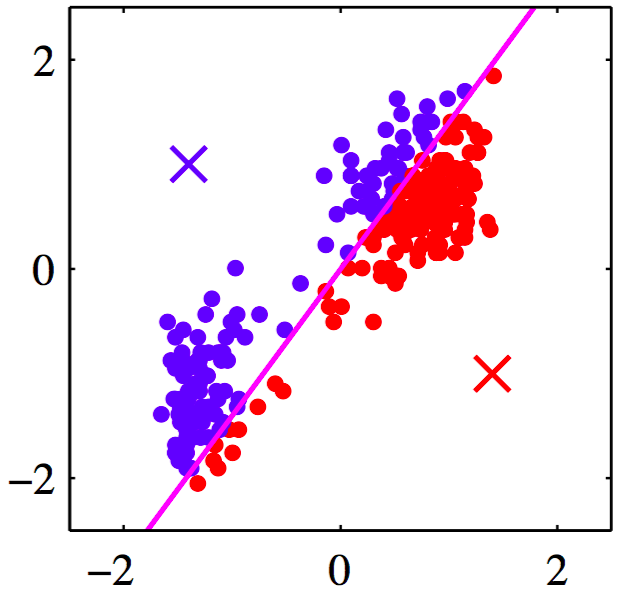
\includegraphics[height=0.55\textheight]{{figures/faithful-9.1b}}
\end{center}

\let\thefootnote\relax\footnotetext{\tiny{From Bishop's \emph{Pattern recognition and machine learning}, Figure 9.1(b).}}
\end{frame}
%
\begin{frame}{$k$-means: by example}

\begin{itemize}
\item Compute new cluster centers.
\end{itemize}
\begin{center}
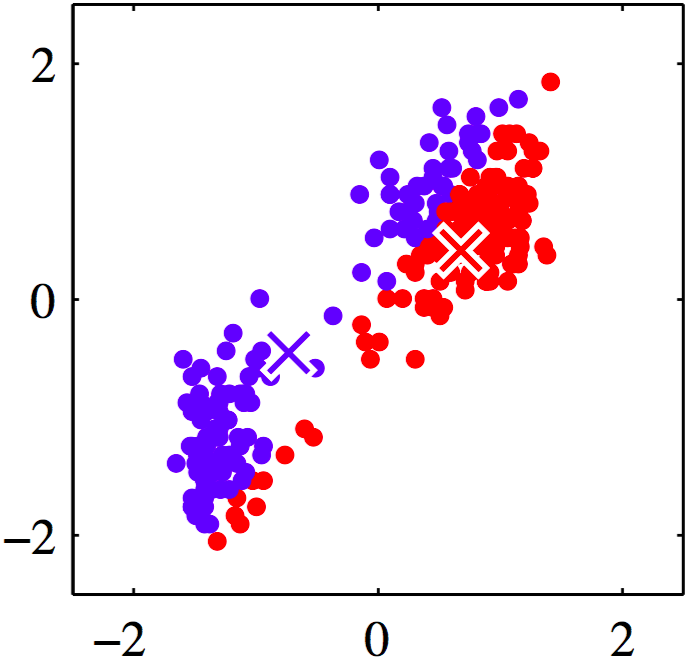
\includegraphics[height=0.55\textheight]{{figures/faithful-9.1c}}
\end{center}

\let\thefootnote\relax\footnotetext{\tiny{From Bishop's \emph{Pattern recognition and machine learning}, Figure 9.1(c).}}
\end{frame}
%
\begin{frame}{$k$-means: by example}

\begin{itemize}
\item Assign points to closest center.
\end{itemize}
\begin{center}
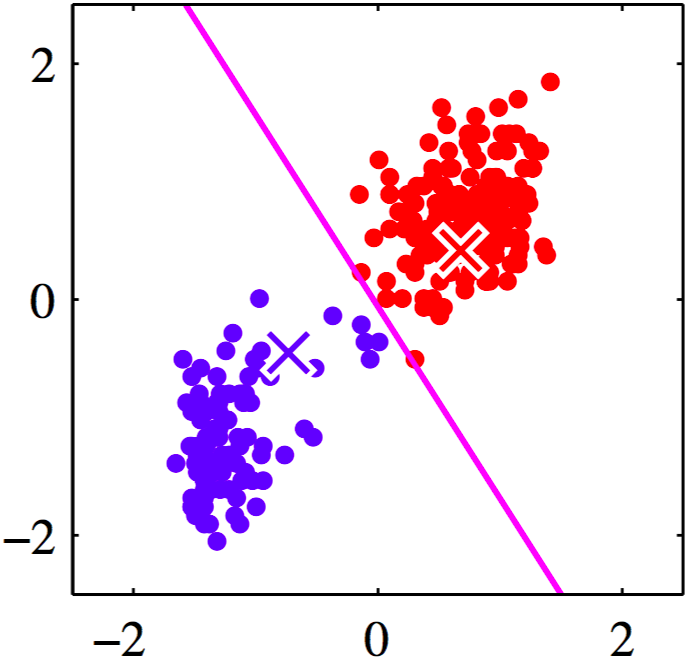
\includegraphics[height=0.55\textheight]{{figures/faithful-9.1d}}
\end{center}

\let\thefootnote\relax\footnotetext{\tiny{From Bishop's \emph{Pattern recognition and machine learning}, Figure 9.1(d).}}
\end{frame}
%
\begin{frame}{$k$-means: by example}

\begin{itemize}
\item Compute cluster centers.
\end{itemize}
\begin{center}
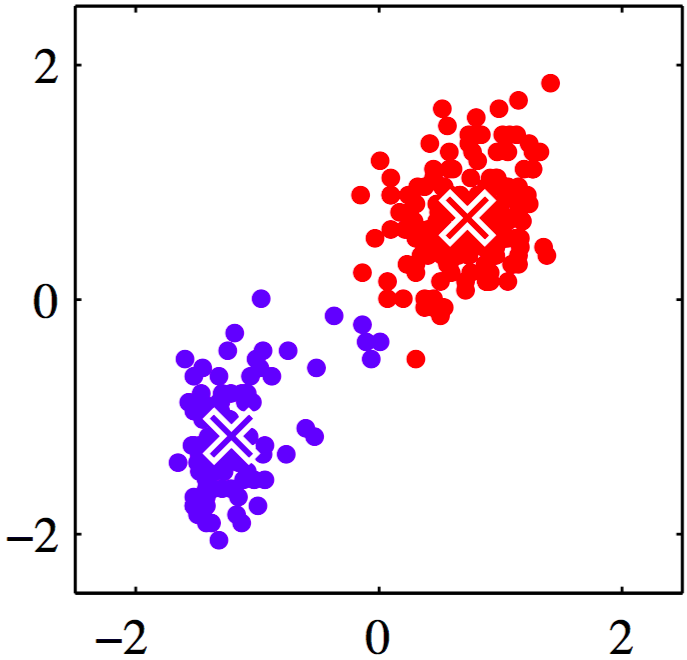
\includegraphics[height=0.55\textheight]{{figures/faithful-9.1e}}
\end{center}

\let\thefootnote\relax\footnotetext{\tiny{From Bishop's \emph{Pattern recognition and machine learning}, Figure 9.1(e).}}
\end{frame}
%
\begin{frame}{$k$-means: by example}

\begin{itemize}
\item Iterate until convergence.
\end{itemize}
\begin{center}
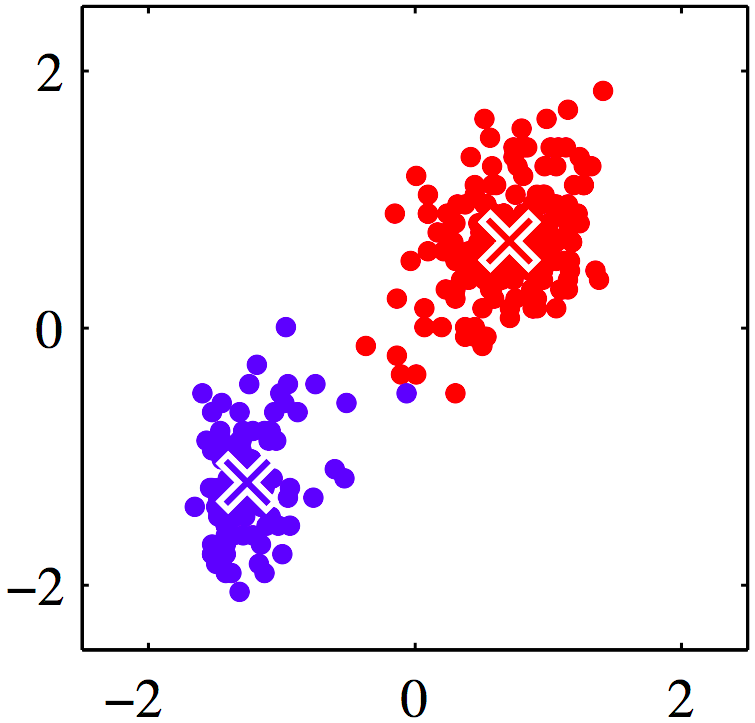
\includegraphics[height=0.55\textheight]{{figures/faithful-9.1i}}
\end{center}

\let\thefootnote\relax\footnotetext{\tiny{From Bishop's \emph{Pattern recognition and machine learning}, Figure 9.1(i).}}
\note[item]{When do we achieve convergence? The cluster assignments no longer change.}
\note[item]{Does it always converge? Yes, more on this later.}
\note[item]{Does it always converge to good clusters? Not necessarily.}
\end{frame}

\begin{frame}{Suboptimal Local Minimum}

\begin{itemize}
\item The clustering for $k=3$ below is a local minimum, but suboptimal:
\end{itemize}
\begin{center}
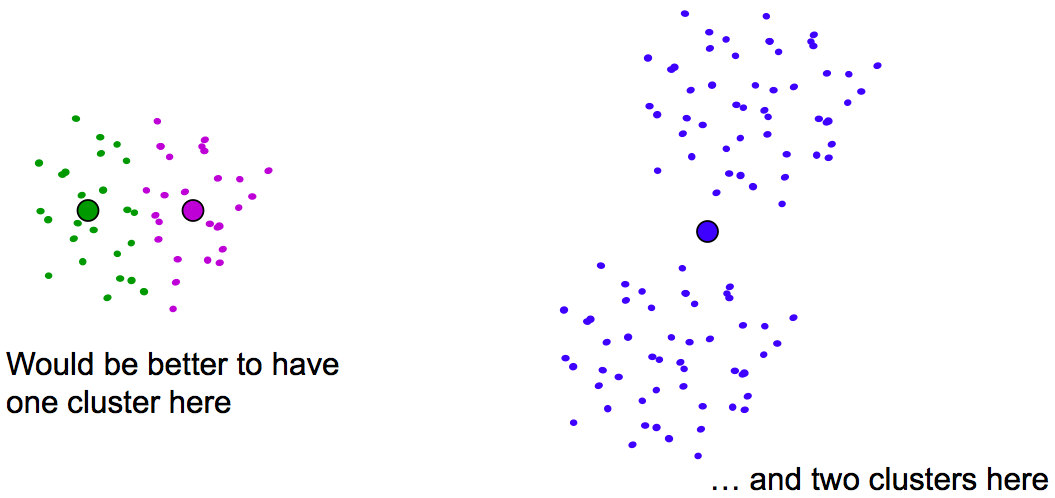
\includegraphics[width=0.8\textwidth]{figures/k-means-local-optimum}\let\thefootnote\relax\footnotetext{\tiny{From Sontag's DS-GA 1003, 2014, Lecture 8.}}
\end{center}
\note[item]{In this example, we have 3 clusters. But $k$-means found different cluster assignments than what we would do. It's a stationary point even though we can find ``better'' clusters.}
\note[item]{How do we define ``good'' clusters? Let's formalize $k$-means with an objective function.}
\end{frame}
%

\begin{frame}{Formalize $k$-Means}
\begin{itemize}[<+->]
\item Dataset $\cd=\left\{ x_{1},\ldots,x_{n}\right\} \subset\cx$ where $\sX = \reals^d$.

\item Goal: Partition data $\cd$ into $k$ disjoint sets $C_{1},\ldots,C_{k}$.
\item Let $c_i \in \pc{1, \ldots, k}$ be the cluster assignment of $x_i$.

\item The \textbf{centroid} of $C_{i}$ is defined to be
\mode<handout>{
\begin{align}
\mu_{i}=\argmin_{\mu\in\cx}\sum_{x\in C_{i}}\|x - \mu\|^{2}.
&& \text{mean of $C_i$}
\end{align}
}
\mode<beamer>{
  \vspace{0.5in}
}

\item The $k$-means objective is to minimize the distance between each example and its cluster centroid:
\mode<handout>{
\begin{align}
J(c, \mu) = \sum_{i=1}^n \| x_i - \mu_{c_i} \|^2 .
\end{align}
}
\mode<beamer>{
  \vspace{0.5in}
}
\end{itemize}
\note[item]{Define the centroid as the point that minimizes its distance to all other points in the cluster. In $\reals^d$,  the distance is Euclidean distance. If you solve this optimization problem, the centroid is the cluster mean.}
\end{frame}

%
\begin{frame}{$k$-Means: Algorithm}
\begin{enumerate}[<+->]
\item Initialize: Randomly choose initial centroids $\mu_{1},\ldots,\mu_{k} \in \reals^d$.

\item Repeat until convergence (i.e. $c_i$ doesn't change anymore):

\begin{enumerate}
\item For all $i$, set
\begin{align}
c_i \leftarrow \argmin_j \| x_i - \mu_j \|^2 .
&& \onslide<6->{\text{Minimize $J$ w.r.t. $c$ while fixing $\mu$}}
\end{align}

\item For all $j$, set 
\begin{align}
\mu_{j} \leftarrow \frac{1}{|C_j|}\sum_{x\in C_j} x .
&& \onslide<7->{\text{Minimze $J$ w.r.t. $\mu$ while fixing $c$.}}
\end{align}
\end{enumerate}
\end{enumerate}
\begin{itemize}
\item<5-> Recall the objective: $J(c, \mu) = \sum_{i=1}^n \| x_i - \mu_{c_i} \|^2$.
%\item<8-> $k$-means is coordinate descent on $J$.
\end{itemize}
\note[item]{Repeat two steps iteratively until convergence. 1) Assign points to their nearest cluster, where the distance is measured by the Euclidean distance between the point and the cluster centroid. 2) Update the cluster centroid given the assignments in the first step.}
\note[item]{Is this algorithm minimizing the objective?}
\note[item]{If we optimize the objective wrt each var while fixing other vars, what is it called?}
\end{frame}
%
\begin{frame}{Avoid bad local minima}
\begin{simpleblock}
{$k$-means converges to a local minimum.}
\begin{itemize}
%\item $k$-means is coordinate descent on $J$, thus $J$ will monotonically decrease.
\item $J$ is non-convex, thus no guarantee to converging to the global minimum.
\end{itemize}
\end{simpleblock}


\begin{simpleblock}
{Avoid getting stuck with bad local minima:}

\begin{itemize}[<+->]
\item Re-run with random initial centroids.
\item \textbf{$k$-means++}: choose initial centroids that spread over all data points.
\begin{itemize}[<+->] 
\item Randomly choose the first centroid from the data points $\cd$.
\item Sequentially choose subsequent centroids from points that are farther away from current centroids:
\begin{itemize}[<+->]
\item Compute distance between each $x_{i}$ and the closest already chosen
centroids.
\item Randomly choose next centroid with probability proportional to the
computed distance squared.
\end{itemize}
\end{itemize}
\end{itemize}
\end{simpleblock}

\note[item]{It can be shown that $k$-means++ converges to a solution not much worse than the optimal solution. Specifically, $\mathbb{E}\pb{J_{k\text{-means}++}} \le O(\log k) J^*$.}
\end{frame}

\begin{frame}
{Summary}
\begin{simpleblock}
{We've seen}
\begin{itemize}
\item Clustering---an unsupervised learning problem that aims to discover group assignments.
\item $k$-means:
\begin{itemize}
\item Algorithm: alternating between assigning points to clusters and computing cluster centroids.
\item Objective: minmizing some loss function by coordinate descent.
\item Converge to a local minimum.
\end{itemize}
\end{itemize}
\end{simpleblock}

\onslide<2->{
\begin{simpleblock}
{Next, probabilistic model of clustering.}
\begin{itemize}
\item A generative model of $x$.
\item Maximum likelihood estimation.
\end{itemize}
\end{simpleblock}
}
\note[item]{At the beginning, we mentioned that unsupervised learning is often formulated as density estimation. But the $k$-means algorithm is not probabilistic. So next let's consider a probabilistic model of clustering and we will show that $k$-means is a special case of this approach.}
\end{frame}

\section{Gaussian Mixture Models}

% \begin{frame}{Probabilistic Model for Clustering}
% \begin{columns}
% % \onslide<1->{
% \begin{column}{0.55\textwidth}
% \begin{itemize}
% \item Problem setup: 
% \begin{itemize}
% \item There are $k$ clusters (or \textbf{mixture components}).
% \item We have a probability distribution for each cluster.
% \end{itemize}
% % \onslide<2->{
% % \item Generative story of a \textbf{mixture distribution}:
% % \begin{enumerate}
% % \item Choose a random cluster $z\in\left\{ 1,2,\ldots,k\right\} $. 
% % \item Choose a point from the distribution for cluster $z$. 
% % \end{enumerate}
% % \end{itemize}
% % }
% \end{column}
% % }
% % \onslide<2->{
% \begin{column}{0.4\textwidth}
% \begin{simpleblock}
% {Example:}
% \begin{enumerate}
% \item Choose $z\in\left\{ 1,2,3\right\} $ with $p(1)=p(2)=p(3)=\frac{1}{3}$. 
% \item Choose $x\mid z\sim\cn\left(X\mid\mu_{z},\Sigma_{z}\right)$.
% \end{enumerate}
% \end{simpleblock}
% 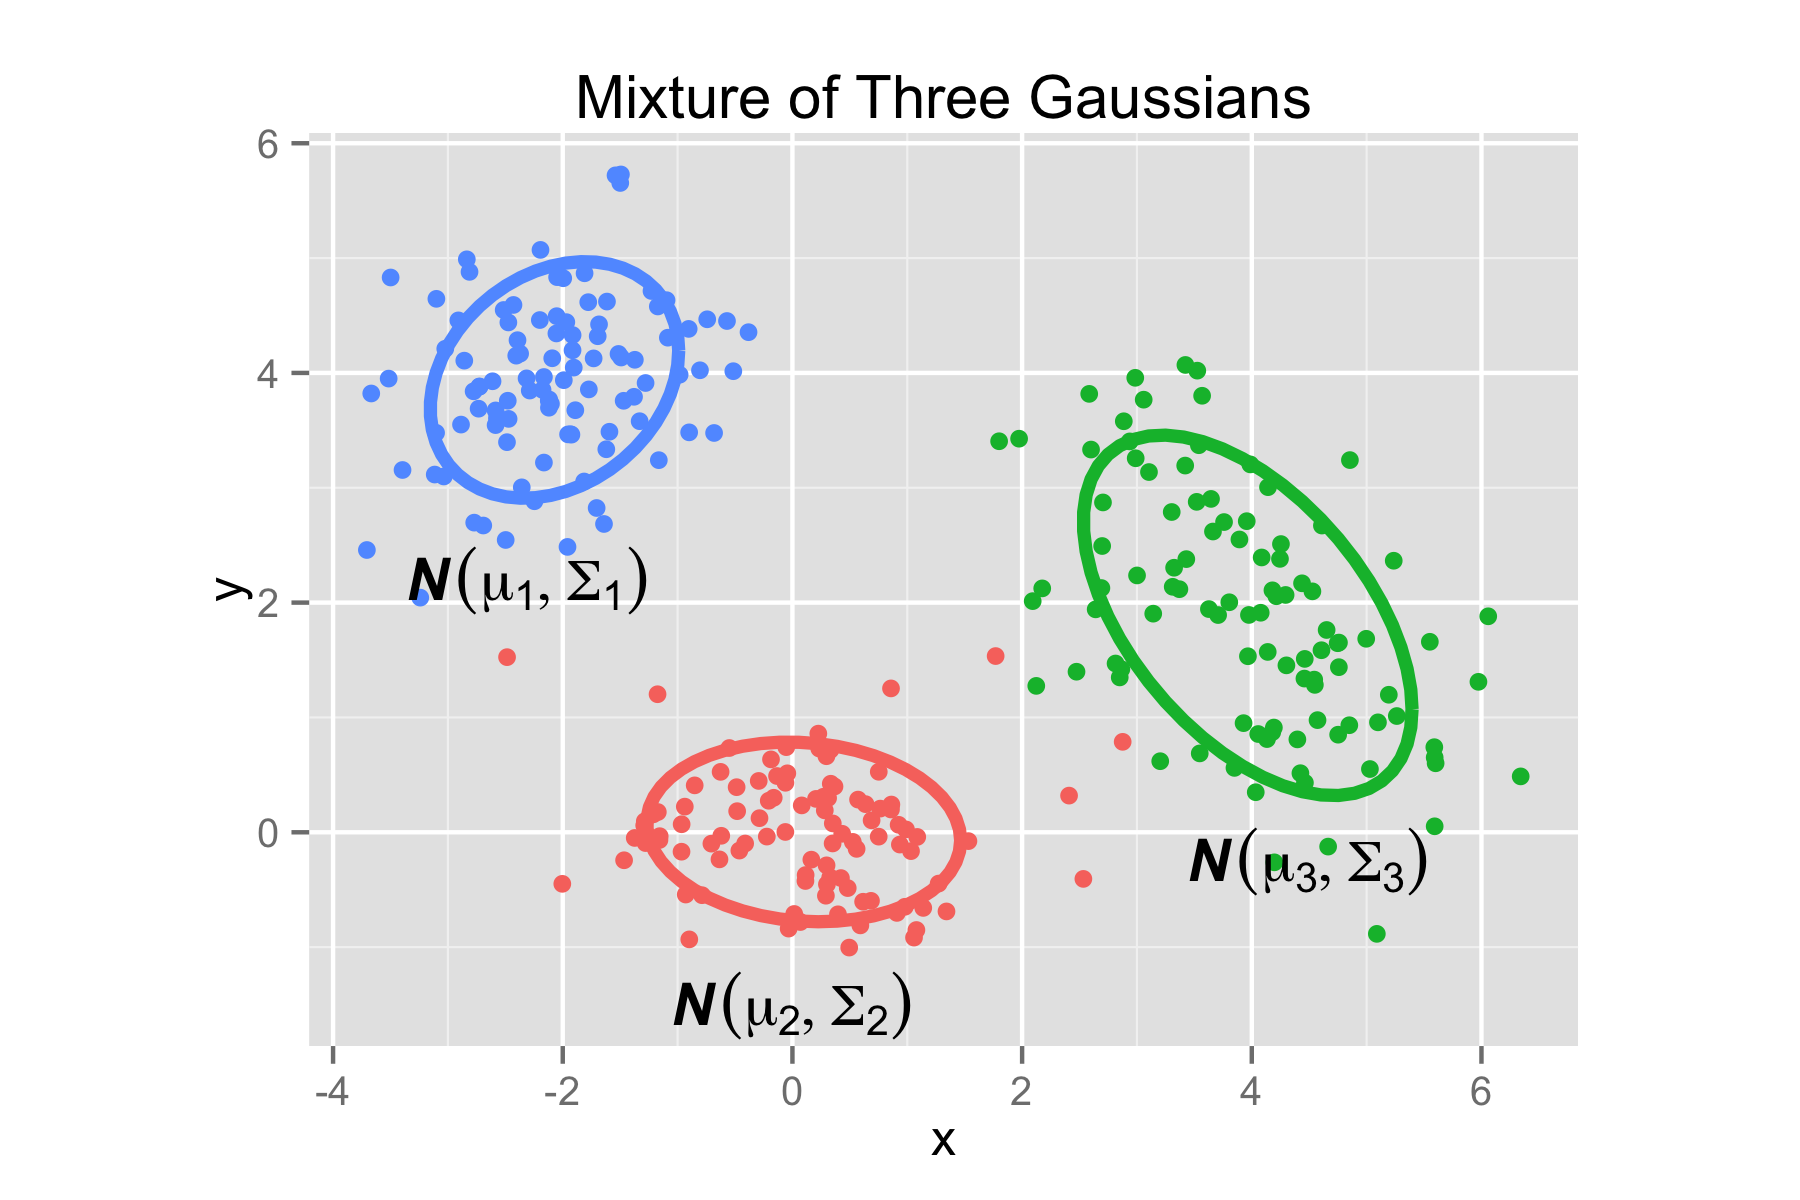
\includegraphics[height=0.5\textheight]{figures/mixture-3-gaussians}
% \end{column}
% % }
% \end{columns}
% \note[item]{Remember that in probabilistic modeling, we want to model the distribution of $p(y\mid x)$ or $p(x, y)$. Here we don't have $y$, so let's model $p(x)$.}
%     \note[item]{So what distribution family should we use to model $x$? Let's think about how $x$ may be generated. It is clear from the figure that there is a two step process. To generate a sample, first, we decide which cluster it comes from, then sample from a distribution of points in that cluster.}
% \end{frame}

\begin{frame}
{Gaussian mixture model (GMM)}
\begin{simpleblock}
{Generative story of GMM with $k$ mixture components:}

\mode<handout>{
\begin{enumerate}
\item Choose cluster $z\sim \text{Categorical}(\pi_1, \ldots, \pi_k)$.
\item Choose $x\mid z \sim \sN(\mu_z, \Sigma_z)$.
\end{enumerate}
}
\mode<beamer>{
  \vspace{0.7in}
}
\end{simpleblock}

\onslide<2->{
\begin{simpleblock}
{Probability density of $x$:}
\begin{itemize}
\item Sum over (marginalize) the \textbf{latent variable} $z$.
\end{itemize}
\mode<handout>{
\begin{align}
\onslide<.->{p(x) &= \sum_z p(x, z) \\}
        \onslide<.->{&= \sum_z p(x\mid z) p(z) \\}
        \onslide<.->{&= \sum_k \pi_k \sN(\mu_k, \Sigma_k)}
\end{align}
}
\mode<beamer>{
  \vspace{1.0in}
}
\end{simpleblock}
}
\note[item]{How do we get the prob density of $x$? We know $p(x\mid z)$ and $p(z)$, which means that we know the joint distribution $p(x,z)$.}
\note[item]{Marginalization: expectation of conditional distribution: $\mathbb{E}_{Y}\pb{X\mid Y} = p(X)$.}
\end{frame}

\begin{frame}{Identifiability Issues for GMM}
\begin{itemize}
\item Suppose we have found parameters 
\begin{eqnarray*}
\text{Cluster probabilities}: &  & \pi=\left(\pi_{1},\ldots,\pi_{k}\right)\\
\text{Cluster means}: &  & \mu=\left(\mu_{1},\ldots,\mu_{k}\right)\\
\text{Cluster covariance matrices:} &  & \Sigma=\left(\Sigma_{1},\ldots\Sigma_{k}\right)
\end{eqnarray*}
 that are at a local minimum.
\end{itemize}

\pause{}
\begin{itemize}
\item What happens if we shuffle the clusters? e.g. Switch the labels for
clusters 1 and 2.
\end{itemize}

\pause{}
\begin{itemize}
\item We'll get the same likelihood. How many such equivalent settings are
there?
\end{itemize}

\pause{}
\begin{itemize}
\item Assuming all clusters are distinct, there are $k!$ equivalent solutions.
\end{itemize}

% \pause{}
% \begin{itemize}
% \item Not a problem \emph{per se}, but something to be aware of.
% \end{itemize}

    \note[item]{We should be careful when interpret the meaning of a cluster. It is tempting to say that cluster 1 is politics, 2 is sports etc. But we will always need to look at the examples in that cluster instead of just relying on the cluster id, which are interchangable.}
\end{frame}

\begin{frame}
{Learning GMMs}
\begin{simpleblock}
{How to learn the parameters $\pi_k, \mu_k, \Sigma_k$?}
\onslide<2->{
\begin{itemize}
\item MLE (also called maximize marginal likelihood).
\item Log likelihood of data:
\mode<handout>{
\begin{align}
L(\theta) &= \sum_{i=1}^n \log p(x_i; \theta) \\
&= \sum_{i=1}^n {\color{red}\log \sum_z} p(x, z; \theta) 
\end{align}
}
\mode<beamer>{
  \vspace{0.8in}
}
}
\onslide<3->{
\item Cannot push $\log$ into the sum... $z$ and $x$ are coupled.
\item No closed-form solution for GMM---try to compute the gradient yourself!
}
\end{itemize}
\end{simpleblock}
\note[item]{Now that we have $p(x)$, how do we learn the parameters of the distribution?}
\note[item]{The log likelihood is just the log probability of the marginals, so it's also called MML when you have latent variables.}
\note[item]{The log sum term is annoying... That means that $z$ and $x$ are coupled and we probably don't have closed form solution. Recall that previously when we take derivative wrt some parameter $\theta_i$, we can ignore all terms whose subscript is not $i$ and the sums would be simplified.}
\end{frame}

\begin{frame}{Gradient Descent / SGD for GMM}
\begin{itemize}
\item What about running gradient descent or SGD on
\begin{eqnarray*}
J(\pi,\mu,\Sigma) & = & -\sum_{i=1}^{n}\log\left\{ \sum_{z=1}^{k}\pi_{z}\cn\left(x_{i}\mid\mu_{z},\Sigma_{z}\right)\right\} ?
\end{eqnarray*}


\pause{}
\item Can be done, in principle -- but need to be clever about it.

\pause{}
\item For example, each covariance matrix $\Sigma_{1},\ldots,\Sigma_{k}$ has to be positive semidefinite.

\pause{}
\item How to maintain that constraint?

\pause{}
\begin{itemize}
\item Rewrite $\Sigma_{i}=M_{i}M_{i}^{T}$, where $M_{i}$ is an unconstrained
matrix. 

\pause{}
\item Then $\Sigma_{i}$ is positive semidefinite. 

\pause{}
\end{itemize}
% \item Even then, pure gradient-based methods have trouble.\footnote{See Hosseini and Sra's \href{https://arxiv.org/abs/1506.07677}{Manifold Optimization for Gaussian Mixture Models}
% for discussion and further references.}
\end{itemize}
\end{frame}


\begin{frame}
{Learning GMMs: observable case}
\begin{simpleblock}
{Suppose we observe cluster assignments $z$. Then MLE is easy:}

\begin{align}
\onslide<1->{
n_{z} &= \sum_{i=1}^{n}\ind{z_{i}=z}
&& \text{\# examples in each cluster}\\
}
\onslide<2->{
\hat{\pi}(z) &= \frac{n_{z}}{n}
&& \text{fraction of examples in each cluster} \\
}
\onslide<3->{
\hat{\mu}_{z} &= \frac{1}{n_{z}}\sum_{i:z_{i}=z}x_{i}
&& \text{empirical cluster mean} \\
}
\onslide<4->{
\hat{\Sigma}_{z} &= \frac{1}{n_{z}}\sum_{i:z_{i}=z}\left(x_{i}-\hat{\mu}_{z}\right)\left(x_{i}-\hat{\mu}_{z}\right)^{T}.
&& \text{empirical cluster covariance}}
\end{align}

\end{simpleblock}
\note[item]{Similar to Gaussian NB where cluster id is like the label of the example.}
\note[item]{How do we know $z$?}
\end{frame}

\begin{frame}
{Learning GMMs: inference}
\begin{simpleblock}
{The inference problem: observe $x$, want to know $z$.}
\mode<handout>{
\begin{align}
% \onslide<2->{p(z=j \mid x_i) &= p(x, z=j) / p(x) \\}
% \onslide<3->{&= \frac{p(x\mid z=j)p(z=j)}{\sum_k p(x\mid z=k) p(z=k)} \\}
% \onslide<4->{&= \frac{\pi_j \sN(x_i \mid \mu_j, \Sigma_j)}{\sum_k \pi_k \sN(x_i \mid \mu_k, \Sigma_k)}}
p(z=j \mid x_i) &= p(x, z=j) / p(x) \\
&= \frac{p(x\mid z=j)p(z=j)}{\sum_k p(x\mid z=k) p(z=k)} \\
&= \frac{\pi_j \sN(x_i \mid \mu_j, \Sigma_j)}{\sum_k \pi_k \sN(x_i \mid \mu_k, \Sigma_k)}
\end{align}
}
\mode<beamer>{
  \vspace{1.0in}
}
\end{simpleblock}
\onslide<2->{
\begin{itemize}
\item $p(z\mid x)$ is a \emph{soft assignment}.
\item If we know the parameters $\mu, \Sigma, \pi$, this would be easy to compute.
\end{itemize}
}
\note[item]{So now we are in a chicken and egg problem. If we know $z$, the parameters are easy to estimate. If we know the problems, $p(z\mid x)$ is easy to estimate.}
\end{frame}

\begin{frame}
{EM for GMM}
Let's compute the cluster assignments and the parameters iteratively.
\onslide<2->{
\begin{simpleblock}
{The expectation-minimization (EM) algorithm:}
\begin{enumerate}
\item Initialize parameters  $\mu, \Sigma, \pi$ randomly.
\item Run until convergence:
}
\begin{enumerate}
\onslide<3->{
\item E-step: fill in latent variables by inference.
\begin{itemize}
\item compute soft assignments $p(z\mid x_i)$ for all $i$.
\end{itemize}
}
\onslide<4->{
\item M-step: standard MLE for $\mu, \Sigma, \pi$ given ``observed'' variables.
\begin{itemize}
\item Equivalent to MLE in the observable case on data weighted by $p(z\mid x_i)$.
}
\end{itemize}
\end{enumerate}
\end{enumerate}
\end{simpleblock}
\end{frame}

\begin{frame}
{M-step for GMM}
\begin{itemize}
%\item {Recall the gradient is:}
%\begin{align}
%\frac{d }{d \theta} \sum_z \log p(x,z;\theta) = \mathbb{E}_{{\color{red}p(z\mid x)}} \pb{ \frac{d}{d\theta}{\color{blue}\log p(x, z)} } 
%\end{align}
\item Let $p(z\mid x)$ be the soft assignments:
\[
    \gamma_{i}^{j}=\frac{\pi_{j}^{\text{old}}\cn\left(x_{i}\mid\mu_{j}^{\text{old}},\Sigma_{j}^{\text{old}}\right)}{\sum_{c=1}^{k}\pi_{c}^{\text{old}}\cn\left(x_{i}\mid\mu_{c}^{\text{old}},\Sigma_{c}^{\text{old}}\right)} .
\]
\item \think{Exercise}: show that
\begin{eqnarray*}
    n_z &=& \sum_{i=1}^n \gamma_i^z \\
\mu_{z}^{\text{new}} & = & \frac{1}{n_{z}}\sum_{i=1}^{n}\gamma_{i}^{z}x_{i}\\
\Sigma_{z}^{\text{new}} & = & \frac{1}{n_{z}}\sum_{i=1}^{n}\gamma_{i}^{z}\left(x_{i}-\mu_{z}^{\text{new}}\right)\left(x_{i}-\mu_{z}^{\text{new}}\right)^{T}\\
\pi_{z}^{\text{new}} & = & \frac{n_{z}}{n} .
\end{eqnarray*}
\end{itemize}
\end{frame}

\begin{frame}{EM for GMM}

\begin{itemize}
\item Initialization
\end{itemize}
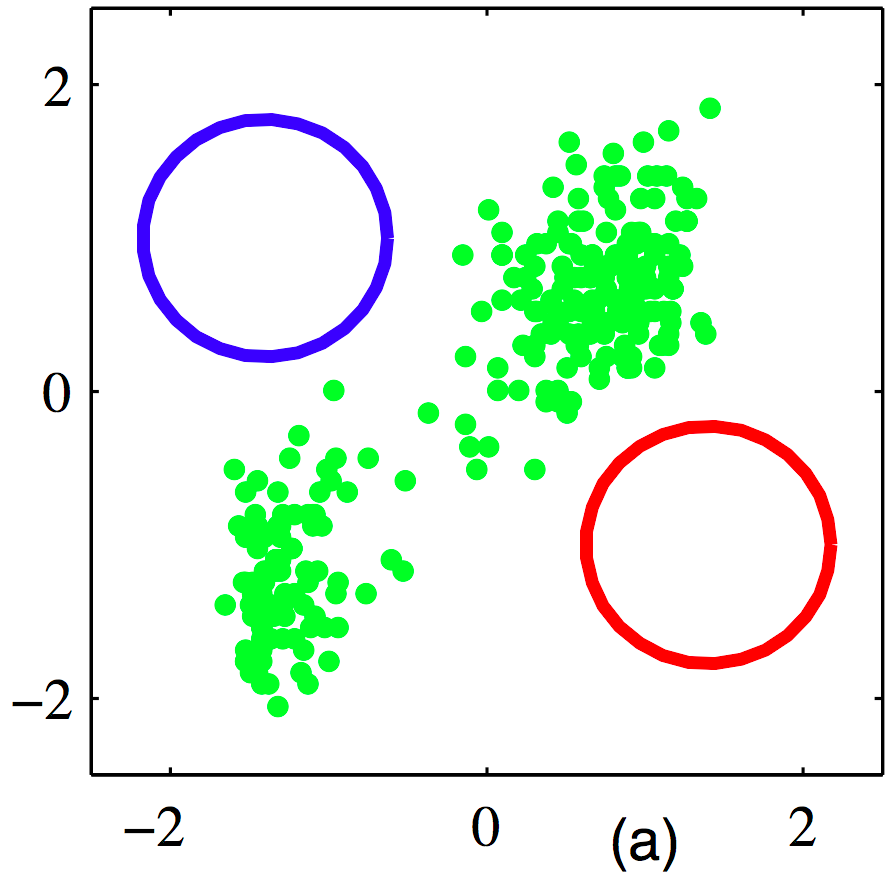
\includegraphics[height=0.55\textheight]{{figures/9.8a}}

\let\thefootnote\relax\footnotetext{\tiny{From Bishop's \emph{Pattern recognition and machine learning}, Figure 9.8.}}
\note[item]{Initially, we have two spherical Gaussian.}
\end{frame}
%
\begin{frame}{EM for GMM}

\begin{itemize}
\item First soft assignment:
\end{itemize}
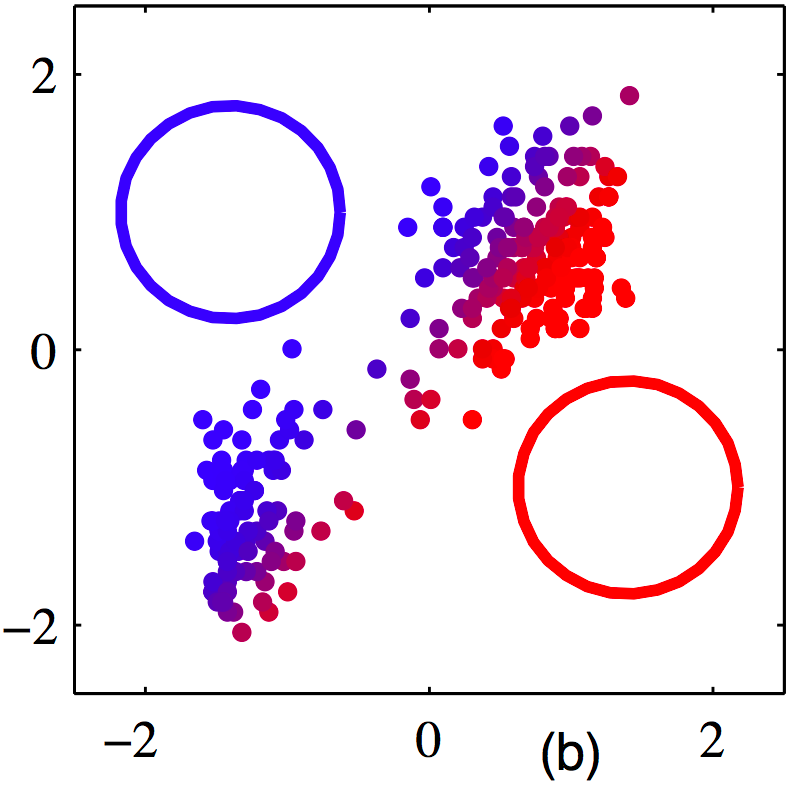
\includegraphics[height=0.55\textheight]{{figures/9.8b}}

\let\thefootnote\relax\footnotetext{\tiny{From Bishop's \emph{Pattern recognition and machine learning}, Figure 9.8.}}
\note[item]{Then we do the soft assignments. The points have mixed cluster membership.}
\end{frame}
%
\begin{frame}{EM for GMM}

\begin{itemize}
\item First soft assignment:
\end{itemize}
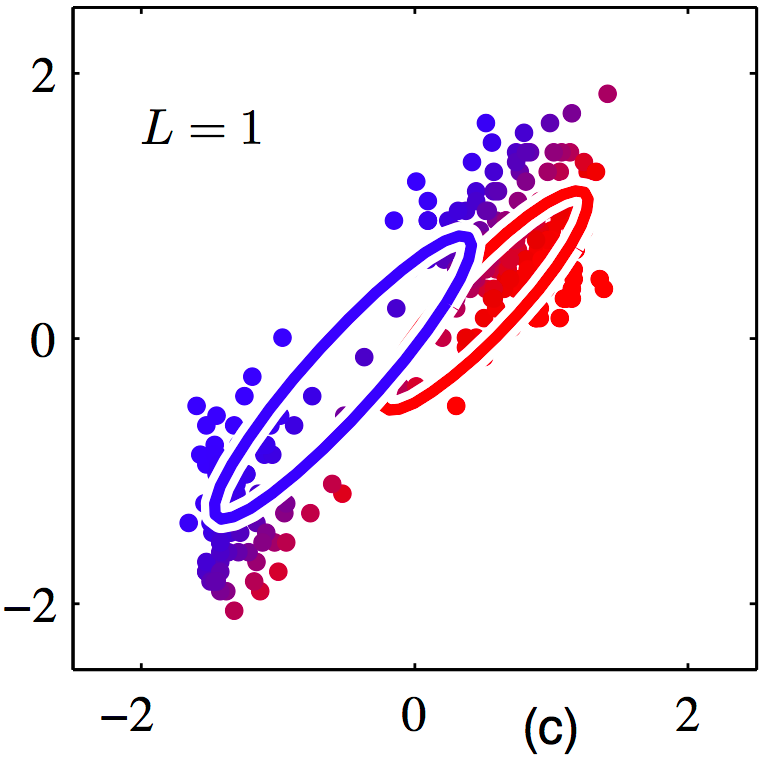
\includegraphics[height=0.55\textheight]{{figures/9.8c}}

\let\thefootnote\relax\footnotetext{\tiny{From Bishop's \emph{Pattern recognition and machine learning}, Figure 9.8.}}
\note[item]{Re-estimate the Gaussians.}
\end{frame}
%
\begin{frame}{EM for GMM}

\begin{itemize}
\item After 5 rounds of EM:
\end{itemize}
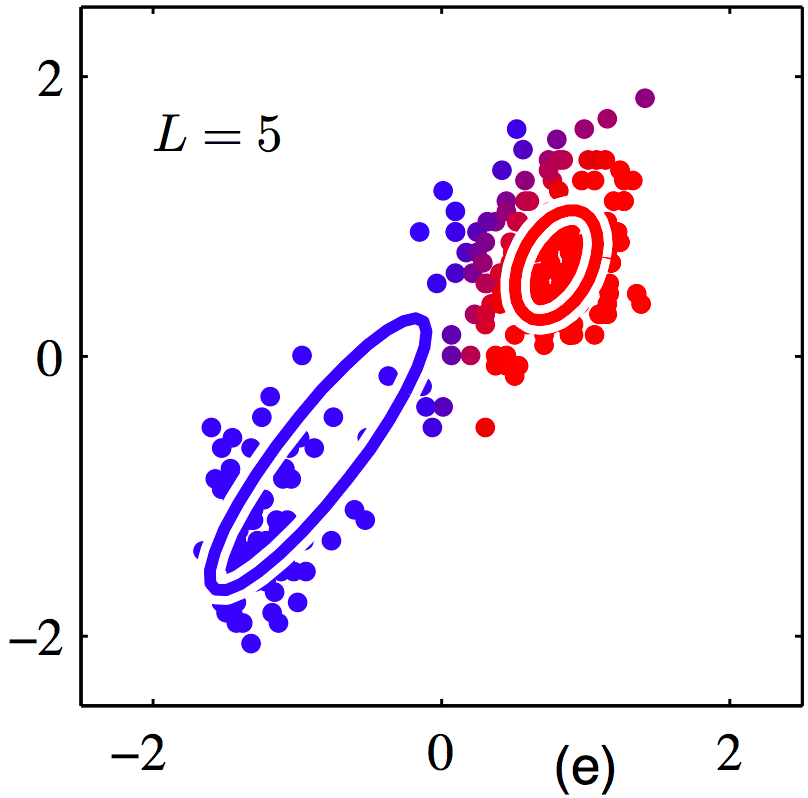
\includegraphics[height=0.55\textheight]{{figures/9.8e}}

\let\thefootnote\relax\footnotetext{\tiny{From Bishop's \emph{Pattern recognition and machine learning}, Figure 9.8.}}

\end{frame}
%
\begin{frame}{EM for GMM}

\begin{itemize}
\item After 20 rounds of EM:
\end{itemize}
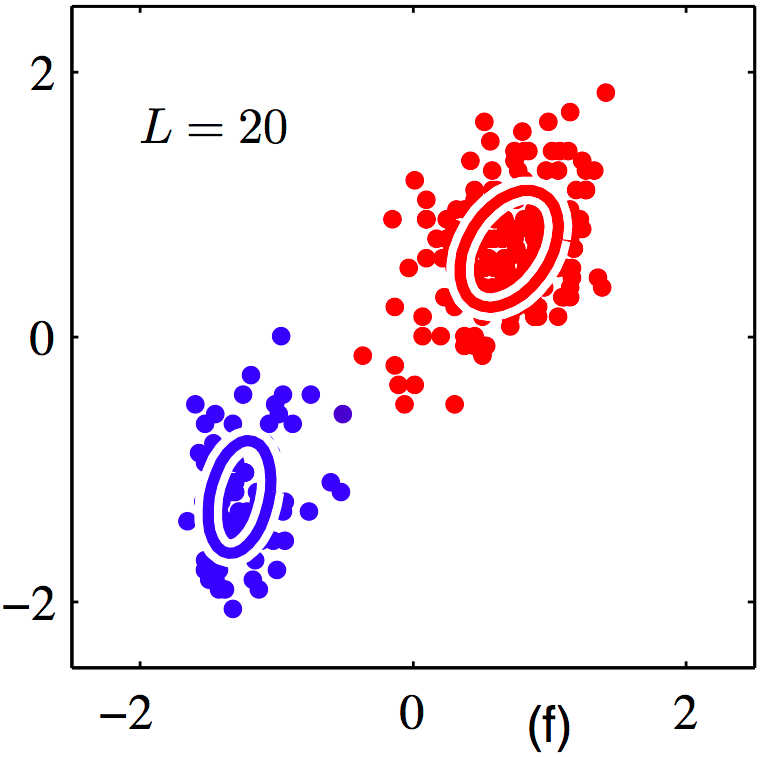
\includegraphics[height=0.55\textheight]{{figures/9.8f}}

\let\thefootnote\relax\footnotetext{\tiny{From Bishop's \emph{Pattern recognition and machine learning}, Figure 9.8.}}
\note[item]{Convergence: likelihood doesn't change much.}
\end{frame}

\begin{frame}
{EM for GMM: Summary}
\begin{itemize}
\item EM is a general algorithm for learning latent variable models.
\item \emph{Key idea}: if data was fully observed, then MLE is easy.
\begin{itemize}
\item E-step: fill in latent variables by computing $p(z\mid x, \theta)$.
\item M-step: standard MLE given fully observed data.
\end{itemize}
\item Simpler and more efficient than gradient methods.
\item Can prove that EM monotonically improves the likelihood and converges to a local minimum.
\item $k$-means is a special case of EM for GMM with \emph{hard assignments}, also called hard-EM.
\end{itemize}
\note[item]{$k$-means: covariance and cluster prior $\pi$ is fixed; only estimate $\mu$; posterior approximated by the delta function.}
\end{frame}

\section{Latent Variable Models }
\begin{frame}{General Latent Variable Model}
\begin{itemize}
\item Two sets of random variables: $z$ and $x$.
\item $z$ consists of unobserved \textbf{hidden variables}.
\item $x$ consists of \textbf{observed variables}.

\pause{}
\item Joint probability model parameterized by $\theta\in\Theta$:
\[
p(x,z\mid\theta)
\]
\end{itemize}

\pause{}
\begin{definition}
A\textbf{ latent variable model }is a probability model for which
certain variables are never observed.

\pause{}

\end{definition}

e.g. The Gaussian mixture model is a latent variable model.
\end{frame}

\begin{frame}{Complete and Incomplete Data}
\begin{itemize}
\item Suppose we observe some data $\left(x_{1},\ldots,x_{n}\right)$.

\pause{}
\item To simplify notation, take $x$ to represent the entire dataset
\[
x=\left(x_{1},\ldots,x_{n}\right),
\]
and $z$ to represent the corresponding unobserved variables
\[
z=\left(z_{1},\ldots,z_{n}\right).
\]
\item An observation of $x$ is called an \textbf{incomplete data set}.
\item An observation $\left(x,z\right)$ is called a \textbf{complete data
set}.
\end{itemize}
\end{frame}
%
 
\begin{frame}{Our Objectives}
\begin{itemize}
\item \textbf{Learning problem}: Given incomplete dataset $x$, find MLE
\[
\hat{\theta}=\argmax_{\theta}p(x\mid\theta).
\]


\pause{}
\item \textbf{Inference problem}: Given $x$, find conditional distribution
over $z$:
\[
p\left(z\mid x,\theta\right).
\]


\pause{}
\item For Gaussian mixture model, learning is hard, inference is easy.
\item For more complicated models, inference can also be hard. %(See DSGA-1005)
\end{itemize}
\end{frame}
%
\begin{frame}{Log-Likelihood and Terminology}
\begin{itemize}
\item Note that
\[
\argmax_{\theta}p(x\mid\theta)=\argmax_{\theta}\left[\log p(x\mid\theta)\right].
\]


\pause{}
\item Often easier to work with this ``\textbf{log-likelihood}''.

\pause{}
\item We often call $p(x)$ the \textbf{marginal likelihood}, 
\begin{itemize}
\item because it is $p(x,z)$ with $z$ ``marginalized out'':
\[
p(x)=\sum_{z}p(x,z)
\]


\pause{}
\end{itemize}
\item We often call $p(x,z)$ the \textbf{joint}. (for ``joint distribution'')

\pause{}
\item Similarly, $\log p(x)$ is the \textbf{marginal log-likelihood}.
\end{itemize}
\end{frame}
%

\section{EM Algorithm}

\begin{frame}
    {Intuition}
    \head{Problem}: marginal log-likelihood $\log p(x;\theta)$ is hard to optimize (observing only $x$)

    \pause
    \head{Observation}: complete data log-likelihood $\log p(x,z;\theta)$ is easy to optimize (observing both $x$ and $z$)

    \pause
    \head{Idea}: guess a distribution of the latent variables $q(z)$ (soft assignments)

    \pause
    Maximize the \textbf{expected complete data log-likelihood}:
    $$
    \max_\theta \sum_{z\in\sZ} q(z) \log p(x,z;\theta)
    $$

    \pause
    \head{EM assumption}: the expected complete data log-likelihood is easy to optimize

    Why should this work?
\end{frame}

\section{Math Prerequisites}

\begin{frame}{Jensen's Inequality}

\begin{theorem}
[Jensen's Inequality]If $f:\reals\to\reals$ is a \textbf{convex}
function, and $x$ is a random variable, then
\[
\ex f(x)\ge f(\ex x).\pause
\]
Moreover, if $f$ is \textbf{strictly convex}, then equality implies
that $x=\ex x$ with probability $1$ (i.e. $x$ is a constant).
\end{theorem}


\pause{}
\begin{itemize}
\item e.g. $f(x)=x^{2}$ is convex. So $\ex x^{2}\ge\left(\ex x\right)^{2}$.
Thus 
\[
\var\left(x\right)=\ex x^{2}-\left(\ex x\right)^{2}\ge0.
\]
 
\end{itemize}
\end{frame}
%
\begin{frame}{Kullback-Leibler Divergence}

\begin{itemize}
\item Let $p(x)$ and $q(x)$ be probability mass functions (PMFs) on $\cx$. 
\item How can we measure how ``different'' $p$ and $q$ are?
\end{itemize}

\pause{}
\begin{itemize}
\item The \textbf{Kullback-Leibler} or \textbf{``KL'' Divergence} is defined
by
\begin{eqnarray*}
\kl(p\|q) & = & \sum_{x\in\cx}p(x)\log\frac{p(x)}{q(x)}.
\end{eqnarray*}
(Assumes $q(x)=0$ implies $p(x)=0$.)
\end{itemize}

\pause{}
\begin{itemize}
\item Can also write this as
\begin{eqnarray*}
\kl(p\|q) & = & \ex_{x\sim p}\log\frac{p(x)}{q(x)}.
\end{eqnarray*}
\end{itemize}
\end{frame}
%
\begin{frame}{Gibbs Inequality ($\kl(p\|q)\ge0$ and $\kl(p\|p)=0$)}
\begin{theorem}
[Gibbs Inequality]Let $p(x)$ and $q(x)$ be PMFs on $\cx$. Then
\[
\kl(p\|q)\ge0,
\]
with equality iff $p(x)=q(x)$ for all $x\in\cx$. 
\end{theorem}


\pause{}
\begin{itemize}
\item KL divergence measures the ``distance'' between distributions.
\end{itemize}

\pause{}
\begin{itemize}
\item Note:

\begin{itemize}
\item KL divergence \textbf{not a metric}.
\item KL divergence is \textbf{not symmetric}.
\end{itemize}
\end{itemize}
\end{frame}
%
\begin{frame}{Gibbs Inequality: Proof}

\begin{eqnarray*}
\kl(p\|q) & = & \ex_{p}\left[-\log\left(\frac{q(x)}{p(x)}\right)\right]\\
 \pause
 & \ge & -\log\left[\ex_{p}\left(\frac{q(x)}{p(x)}\right)\right]\mbox{\qquad\text{(Jensen's)}}\\
 \pause
 & = & -\log\left[\sum_{\left\{ x\mid p(x)>0\right\} }p(x)\frac{q(x)}{p(x)}\right]\\
 \pause
 & = & -\log\left[\sum_{x\in\cx}q(x)\right]\\
 \pause
 & = & -\log1=0.
\end{eqnarray*}


\pause{}
\begin{itemize}
\item Since $-\log$ is strictly convex, we have strict equality iff $q(x)/p(x)$
is a constant, which implies $q=p$ . 
\end{itemize}
\end{frame}

\section{The ELBO: Family of Lower Bounds on $\log p(x\mid\theta)$}
\begin{frame}{The Maximum Likelihood Estimator}

\mode<handout>{
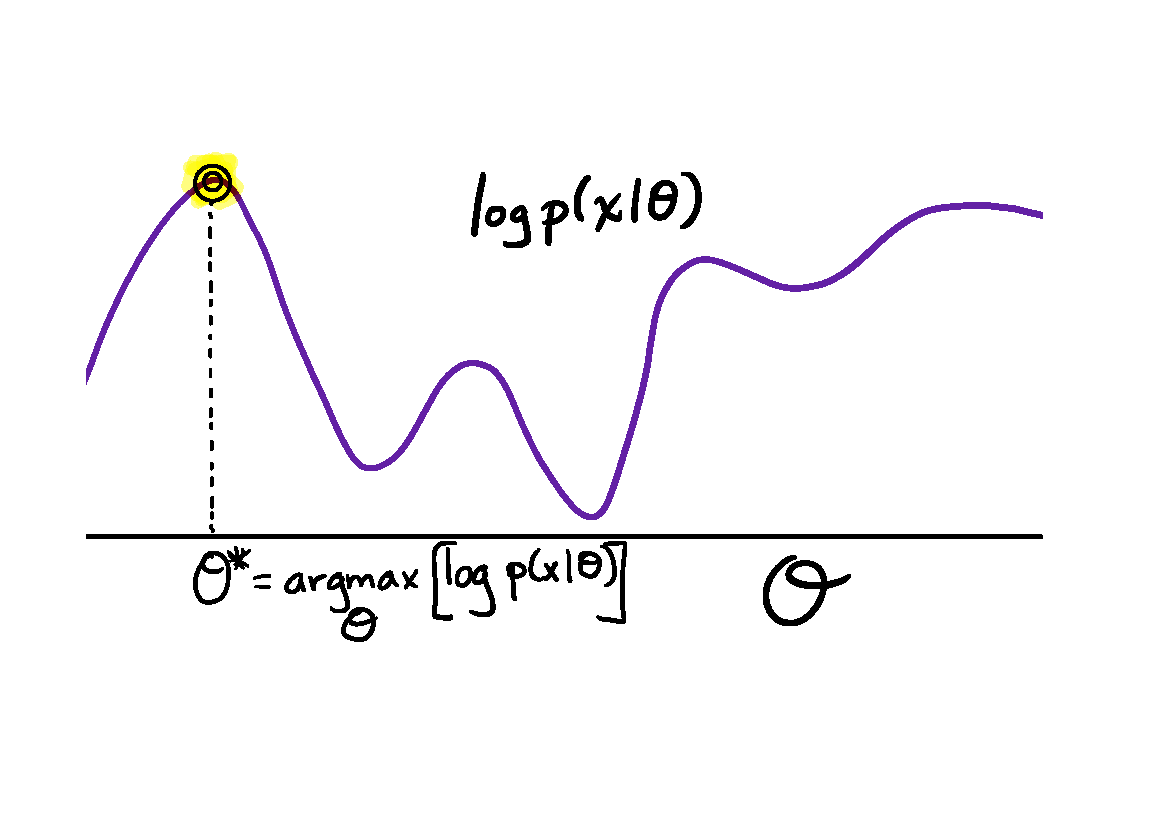
\includegraphics[width=0.85\textwidth]{figures/margLL-withMax.pdf}
}
    \note[item]{To give an overivew of the EM algorithm, let's use this 1-d illustration. The marginal log-likelihood is a complex non-convex function, and we would like to find the parameter  that maximizes the marginal log-likelihood. Because it's hard to directly maximize this function, we will maximize its lower bound instead. Now, there can be many possible lowerbounds, some are useless (example). The key of the EM algorithm is to construct "good" lowerbounds which are easy to optimize and tight, meaning if you optimize the lower bound you also optimize the true function.}
\end{frame}

\begin{frame}
    {Lower bound of the marginal log-likelihood}
    \mode<handout>{
    \begin{eqnarray*}
        \log p(x;\theta) & = & \log \sum_{z\in\sZ} p(x,z;\theta) \\
        \pause
        &=& \log \sum_{z\in\sZ} q(z) \frac{p(x,z;\theta)}{q(z)}\\
        \pause
        %\quad {\color{brown}= \log \BE_z\pb{p(x,z;\theta)}}\\
        &\ge& \sum_{z\in\sZ} q(z) \log \frac{p(x,z;\theta)}{q(z)}\\
        \pause
        %\quad {\color{brown}= \BE_z\pb{\log p(x,z;\theta)}} \\
        &\eqdef& \sL(q, \theta)
    \end{eqnarray*}
    \vspace{-2em}
    \begin{itemize}
        \setlength\itemsep{2pt}
        \item \textbf{Evidence}:  $\log p(x;\theta)$
        \item \textbf{Evidence lower bound (ELBO)}: $\sL(q, \theta)$
        \item $q$: chosen to be a family of tractable distributions
        \item Idea: \emph{maximize the ELBO} instead of $\log p(x;\theta)$
    \end{itemize}
    }
\end{frame}

\begin{frame}{MLE, EM, and the ELBO}
\begin{itemize}
\item<+-> The MLE is defined as a maximum over $\theta$:
\[
\hat{\theta}_{\text{MLE}}=\argmax_{\theta}\left[\log p(x\mid\theta)\right].
\]
\item<+-> For any PMF $q(z)$, we have a lower bound on the marginal log-likelihood
\[
\log p(x\mid\theta)\ge\cl(q,\theta).
\]
\item<+-> In EM algorithm, we maximize the lower bound (ELBO) over $\theta$
and $q$:
\[
\hat{\theta}_{\text{EM}}\approx\argmax_{\theta}\left[\max_{q}\cl(q,\theta)\right]
\]
% \end{itemize}
% \pause{}
% \begin{itemize}
\item<+-> In EM algorithm, $q$ ranges over all distributions on $z$.
\end{itemize}
\end{frame}

\begin{frame}{EM: Coordinate Ascent on Lower Bound}
\begin{itemize}
\item Choose sequence of $q$'s and $\theta$'s by ``\textbf{coordinate
ascent}'' on $\cl(q,\theta)$.

\pause{}
\item EM Algorithm (high level):
\begin{enumerate}
\item Choose initial $\theta^{\text{old}}$.
\item Let $q^{*}=\argmax_{q}\cl(q,\theta^{\text{old}})$

\pause{}
\item Let $\theta^{\text{new}}=\argmax_{\theta}\cl(q^{*},\theta)$.

\pause{}
\item Go to step 2, until converged.
\end{enumerate}
\item Will show:\textbf{ $p(x\mid\theta^{\text{new}})\ge p(x\mid\theta^{\text{old}})$}
\item \textbf{Get sequence of $\theta$'s with monotonically increasing
likelihood.}
\end{itemize}
\end{frame}

\begin{frame}{EM: Coordinate Ascent on Lower Bound}
\begin{center}
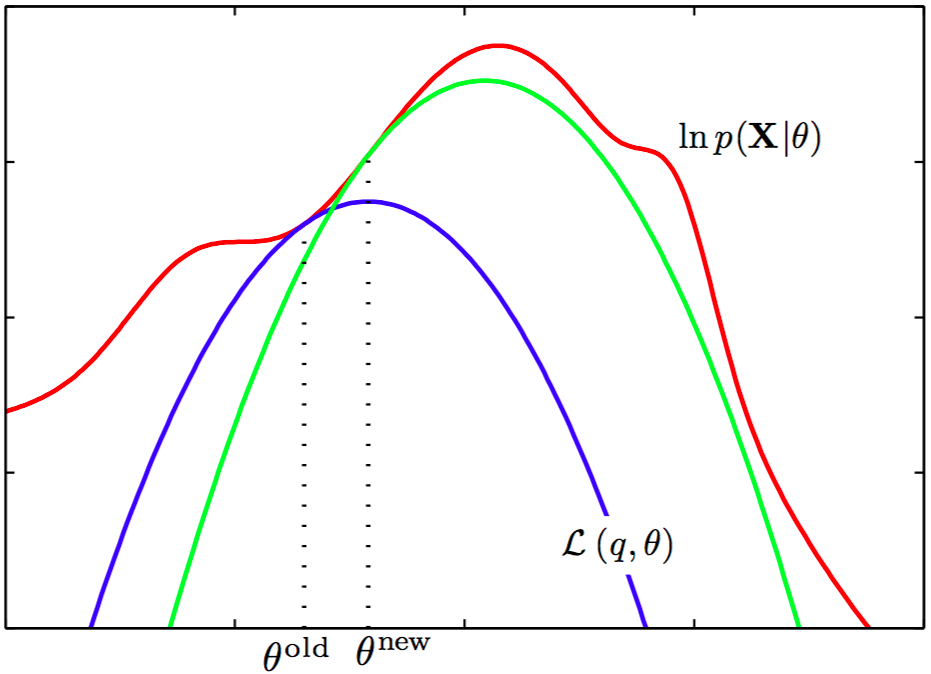
\includegraphics[height=0.5\textheight]{figures/EM-twosteps-Bishop9.14.png} 
\par\end{center}
\begin{enumerate}
\item Start at $\theta^{\text{old}}.$ 

\pause{}
\item Find $q$ giving best lower bound at $\theta^{\text{old}}$$\implies$
$\cl(q,\theta)$. 

\pause{}
\item $\theta^{\text{new}}=\argmax_{\theta}\cl(q,\theta)$.
\end{enumerate}
\let\thefootnote\relax\footnotetext{\tiny{From Bishop's \emph{Pattern recognition and machine learning}, Figure 9.14.}}
\end{frame}

\begin{frame}
    {Is ELBO a "good" lowerbound?}
    \begin{align*}
        \sL(q, \theta) &= \sum_{z\in\sZ} q(z) \log \frac{p(x,z \mid\theta)}{q(z)} \\
        &= \sum_{z\in\sZ} q(z)\log \frac{p(z\mid x,\theta)p(x\mid\theta)}{q(z)} \\
        &= -\sum_{z\in\sZ}q(z) \log \frac{q(z)}{p(z\mid x,\theta)}
        + \sum_{z\in\sZ} q(z) \log p(x\mid\theta) \\
        &= -\KL{q(z)}{p(z\mid x,\theta)} + \underbrace{\log p(x\mid\theta)}_{\text{evidence}}
    \end{align*}
    \vspace{-2em}
    \begin{itemize}
        \item \textbf{KL divergence}: measures ``distance'' between two distributions (not symmetric!)
        \item $\KL{q}{p}\ge 0$ with equality iff $q(z) = p(z\mid x)$.
        \item ELBO = evidence - KL $\le$ evidence
    \end{itemize}
\end{frame}

\begin{frame}{Maximizing over $q$ for fixed $\theta$.}
\begin{itemize}
\item Find $q$ maximizing
\begin{eqnarray*}
\cl(q,\theta) & = & -\kl[q(z),p(z\mid x,\theta)]+\underbrace{\log p(x\mid\theta)\pause}_{\text{no }q\text{ here}}
\end{eqnarray*}


\pause{}
\item Recall $\kl(p\|q)\ge0$, and $\kl(p\|p)=0$.

\pause{}
\item Best $q$ is $q^{*}(z)=p(z\mid x,\theta)$ and
\[
\pause\cl(q^{*},\theta)=-\underbrace{\kl[p(z\mid x,\theta),p(z\mid x,\theta)]}_{=0}+\log p(x\mid\theta)
\]


\pause{}
\item Summary:
\[
\log p(x\mid\theta)=\sup_{q}\cl(q,\theta)\qquad\forall\theta
\]
\item For any $\theta$, \textbf{sup is attained} at $q(z)=p(z\mid x,\theta)$. 
\end{itemize}
\end{frame}
%

%\begin{frame}
%    {\dis Justification for maximizing ELBO}
%    $
%    \sL(q, \theta) = -\KL{q(z)}{p(z\mid x;\theta)} + \log p(x;\theta)
%    $
%
%    Fix $\theta=\theta_0$ and $\max_q \sL(q, \theta_0)$: $q^* = p(z\mid x;\theta_0)$ 
%    \vspace{10em}
%
%    Let $\theta^*, q^*$ be the global optimzer of $\sL(q, \theta)$, then $\theta^*$ is the global optimizer of $\log p(x;\theta)$. (Proof: exercise)
%\end{frame}

\begin{frame}{Marginal Log-Likelihood \textbf{IS}\textbf{\textcolor{blue}{\LARGE{}
}}the Supremum over Lower Bounds}

\mode<handout>{
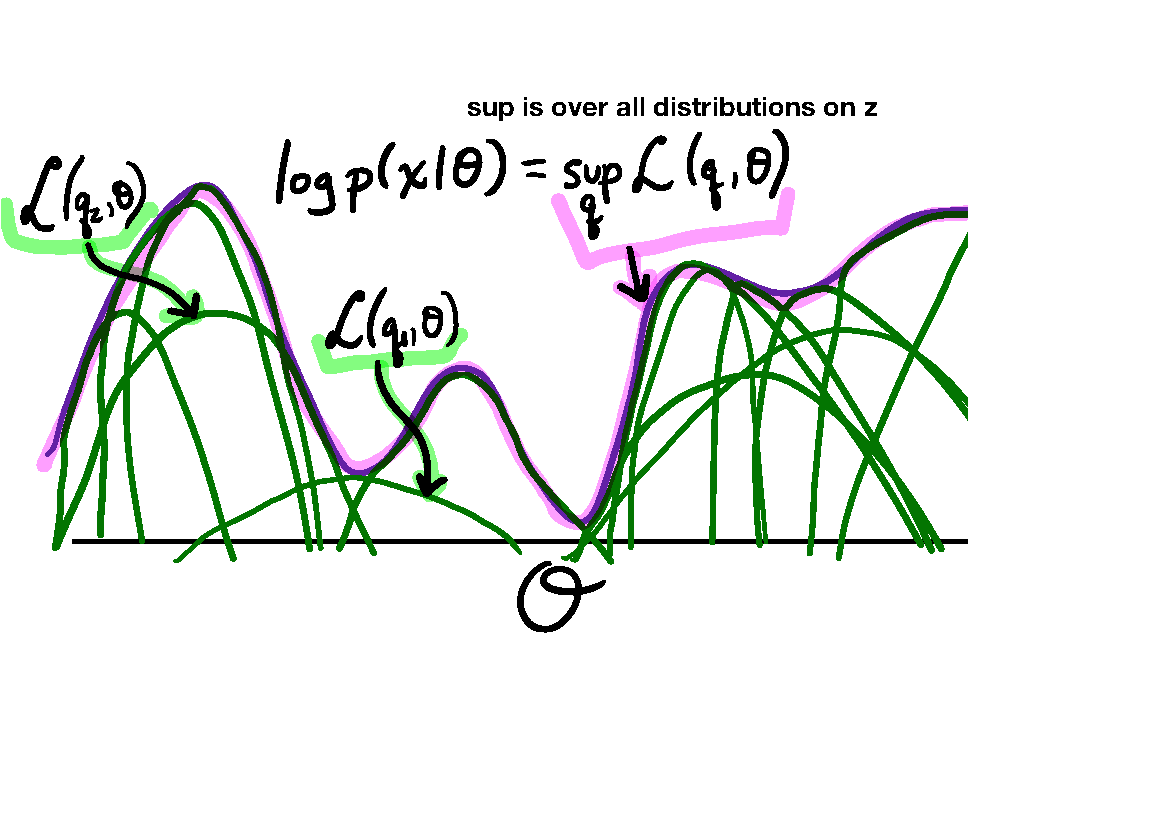
\includegraphics[width=0.75\textwidth]{figures/sup-margLL.pdf} 
}
\end{frame}

\begin{frame}
    {Summary}
    \textbf{Latent variable models}: clustering, latent structure, missing lables etc.

    \head{Parameter estimation}: maximum marginal log-likelihood

    \head{Challenge}: directly maximize the \textbf{evidence} $\log p(x;\theta)$ is hard

    \head{Solution}: maximize the \textbf{evidence lower bound}:
    $$
    \text{ELBO} = \sL(q, \theta) = -\KL{q(z)}{p(z\mid x;\theta)} + \log p(x;\theta)
    $$

    \head{Why does it work?}
    \begin{align*}
        q^*(z) &= p(z\mid x; \theta) \quad \forall \theta \in \Theta \\
        \sL(q^*, \theta^*) &= \max_\theta \log p(x; \theta)
    \end{align*}
\end{frame}

\begin{frame}
    {EM algorithm}
    \emph{Coordinate ascent on $\sL(q, \theta)$}\\
    \begin{enumerate}
        \item Random initialization: $\theta^{\text{old}} \leftarrow \theta_0$
        \item Repeat until convergence
            \begin{enumerate}[(i)]
                \item $q(z) \leftarrow \argmax_q \sL(q, \theta^{\text{old}})$
                    \begin{align*}
                    \text{\textbf{Expectation} (the E-step):} \quad
                    q^*(z) &= p(z\mid x;\theta^{\text{old}}) \\
                        J(\theta) &= \sL(q^*, \theta) 
                    \end{align*}
                \item $\theta^{\text{new}} \leftarrow \argmax_\theta \sL(q^*, \theta)$
                    \begin{align*}
                        \text{\textbf{Maximization} (the M-step):} \quad
                        \theta^{\text{new}} \leftarrow \argmax_\theta J(\theta)
                    \end{align*}
            \end{enumerate}
    \end{enumerate}
\end{frame}

\begin{frame}{EM Algorithm}
\begin{enumerate}
%\item Choose initial $\theta^{\text{old}}$.
\item \textbf{Expectation Step}
\begin{itemize}
    \setlength\itemsep{1pt}
\item Let $q^{*}(z)=p(z\mid x,\theta^{\text{old}})$. {[}$q^{*}$ gives
best lower bound at $\theta^{\text{old}}${]}

\pause{}
\item Let
\[
J(\theta):=\cl(q^{*},\theta)=\underbrace{\sum_{z}q^{*}(z)\log\left(\frac{p(x,z\mid\theta)}{q^{*}(z)}\right)}_{\mbox{\textbf{expectation }w.r.t. }z\sim q^{*}(z)}
\]
 

\pause{}
\end{itemize}
\item \textbf{Maximization Step} 
\[
\theta^{\text{new}}=\argmax_{\theta}J(\theta).\pause
\]
{[}Equivalent to maximizing expected complete log-likelihood.{]}

\pause{}
%\item Go to step 2, until converged.
\end{enumerate}
        EM puts no constraint on $q$ in the E-step and assumes the M-step is easy.
        In general, both steps can be hard.
\end{frame}

\begin{frame}
    {Monotonically increasing likelihood}
    \begin{figure}
        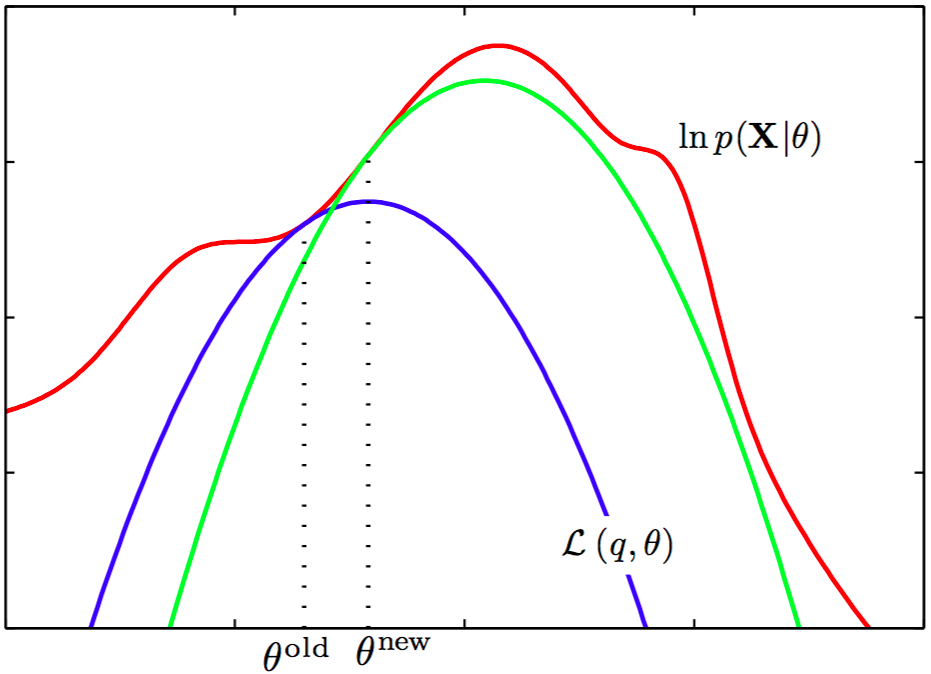
\includegraphics[height=5cm]{figures/EM-twosteps-Bishop9.14.png}
    \end{figure}
    \vspace{-2em}
    Exercise: prove that EM increases the marginal likelihood monotonically
    $$
    \log p(x;\theta^{\text{new}}) \ge \log p(x;\theta^{\text{old}})
    \;.
    $$
    Does EM converge to a global maximum?

    \note[item]{$\log p(x, \theta_o) = \sL(q^*, \theta_o) \le \sL(q^*, \theta_n) \le \log p(x, \theta_n)$}
\end{frame}

\section{Variations on EM}

\begin{frame}{EM Gives Us Two New Problems}
\begin{itemize}
\item The ``E'' Step: Computing

\[
J(\theta):=\cl(q^{*},\theta)=\sum_{z}q^{*}(z)\log\left(\frac{p(x,z\mid\theta)}{q^{*}(z)}\right)
\]


\pause{}
\item The ``M'' Step: Computing
\[
\theta^{\text{new}}=\argmax_{\theta}J(\theta).\pause
\]


\pause{}
\item Either of these can be too hard to do in practice.
\end{itemize}
\end{frame}

\begin{frame}{Generalized EM (GEM)}
\begin{itemize}
\item Addresses the problem of a difficult ``M'' step.

\pause{}
\item Rather than finding 
\[
\theta^{\text{new}}=\argmax_{\theta}J(\theta),
\]
find \textbf{any} $\theta^{\mbox{new}}$ for which
\[
J(\theta^{\mbox{new}})>J(\theta^{\mbox{old}}).
\]


\pause{}
\item Can use a standard nonlinear optimization strategy
\begin{itemize}
\item e.g. take a gradient step on $J$.

\pause{}
\end{itemize}
\item We still get monotonically increasing likelihood. 
\end{itemize}
\end{frame}

\begin{frame}{EM and More General Variational Methods}
\begin{itemize}
\item Suppose ``E'' step is difficult:
\begin{itemize}
\item Hard to take expectation w.r.t. $q^{*}(z)=p(z\mid x,\theta^{\text{old}})$.
\end{itemize}

\pause{}
\item Solution: Restrict to distributions $\cq$ that are easy to work with. 

\pause{}
\item Lower bound now looser:
\[
q^{*}=\argmin_{q\in\cq}\kl[q(z),p(z\mid x,\theta^{\text{old}})]
\]
\end{itemize}
\end{frame}

\begin{frame}{Deep Latent Variable Models}
\begin{columns}
\begin{column}{0.54\textwidth}
\begin{itemize}
  \item<+-> Neural network is a flexible function class to represent transformation between random variables $\eg q(z)$.
  \item<+-> In neural networks, the hidden activations do not have probabilistic interpretation as they are not random variables.
  \item<+-> What if we let the hidden represent some learned latent code?
\end{itemize}
\end{column}
\begin{column}{0.45\textwidth}
\begin{center}
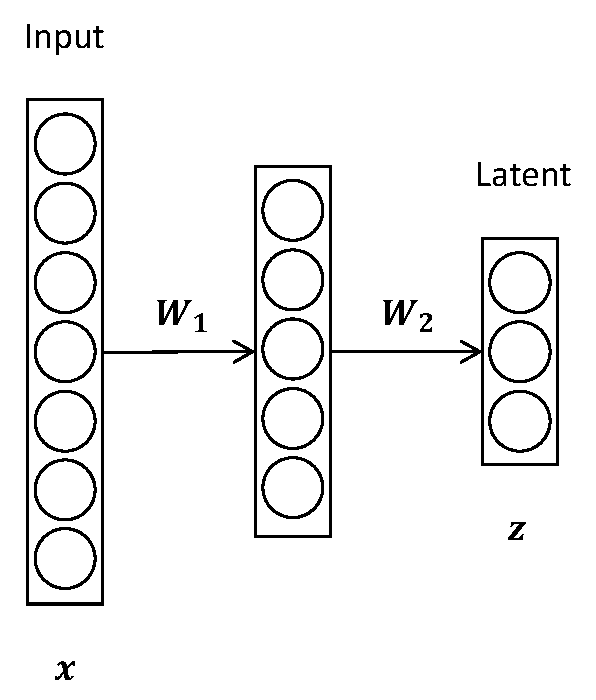
\includegraphics[width=0.7\textwidth]{figures/deep-latent.pdf}
\end{center}
\end{column}
\end{columns}
\end{frame}

\begin{frame}{Variational Autoencoders (VAE) \footnote{\tiny Diederik P Kingma, Max Welling. Auto-Encoding Variational Bayes. ICLR 2014.}}
\begin{itemize}
  \item<+-> An autoencoder (AE) is a neural network that reconstructs the same input.
  \item<+-> The first half is an encoder, from input to latent. The second half is a decoder.
  \item<+-> How to make $q$ a probability distribution?
\end{itemize}
\begin{center}
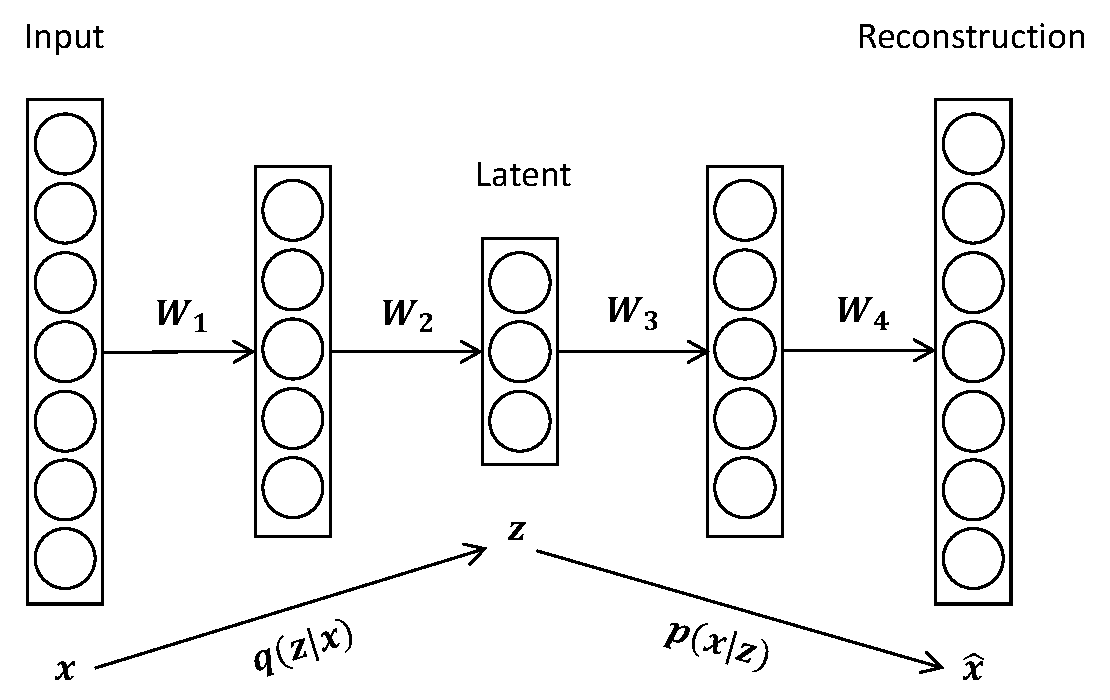
\includegraphics[width=0.4\textwidth]{figures/vae.pdf}
\end{center}
\end{frame}

\begin{frame}{Reparameterization Trick}
\begin{columns}
\begin{column}{0.5\textwidth}
\begin{itemize}
  \item<+-> Let's assume that $q(z|x)$ is a Gaussian distribution.
  \item<+-> Instead of letting the neural network to output a stochastic variable, we can let it predict deterministically the distribution parameters $\mu$ and $\sigma$.
  \item<+-> A stochastic $z$ can be sampled from $\mathcal{N}(\mu, \sigma^2)$: $z = \mu + \sigma \cdot \epsilon$, where $\epsilon \sim \mathcal{N}(0, 1).$
\end{itemize}
\end{column}
\begin{column}{0.5\textwidth}
\begin{center}
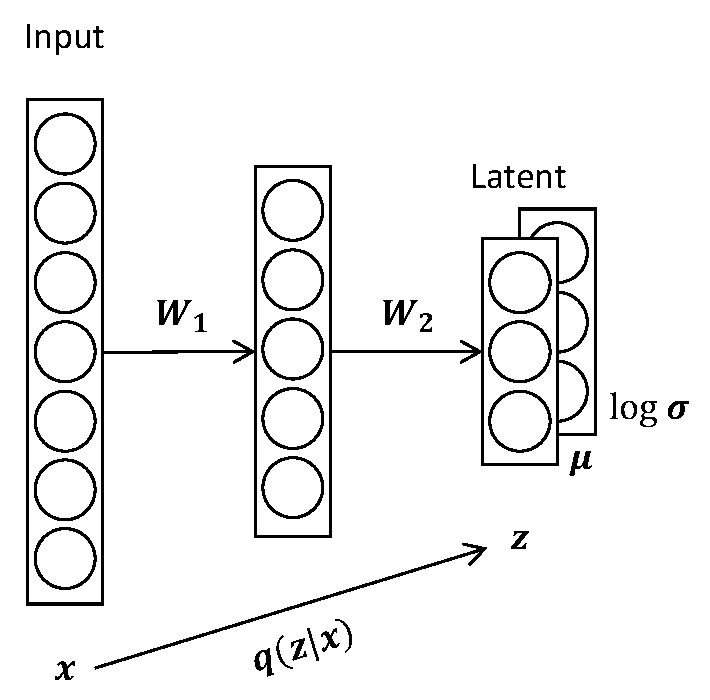
\includegraphics[width=0.7\textwidth]{figures/vae-reparameterization.pdf}
\end{center}
\end{column}
\end{columns}
\end{frame}

\begin{frame}{Variational Lower Bound}
\begin{itemize}
  \item<+-> Encoder $q$ weights: $\phi$; Decoder $p$ weights: $\theta$.
  \item<+-> Now maximize ELBO: 
  \begin{align}
  \onslide<3->{L(q; \phi, \theta) &= \sum_{z} q(z) \log \frac{p_\theta(x, z)}{q_\phi(z|x)} \\}
  \onslide<4->{&= \mathbb{E}_{z \sim q} [-\log q_\phi(z|x) + \log p_\theta(x, z)] \\}
  \onslide<5->{&= \mathbb{E}_{z \sim q} [-\log q_\phi(z|x) + \log p_\theta(x | z) + \log p_\theta(z)] \\}
  \onslide<6->{&= \underbrace{-KL(q_\phi(z|x) || p_\theta(z))}_{\text{Divergence between }q\text{ and the prior distribution}} + \underbrace{\mathbb{E}_{z \sim q}(\log p_\theta(x | z))}_{\text{Reconstruction based on }z}}
  \end{align}
\end{itemize}
\end{frame}

\begin{frame}{Stochastic Gradient}
\begin{itemize}
  \item<+-> The loss function needs to take expectation over $q$:
  \[
   L(q; \phi, \theta) = -KL(q_\phi(z|x) || p_\theta(z)) + \mathbb{E}_{z \sim q}(\log p_\theta(x | z))
   \]
  \item<+-> Turns out we just need to have a Monte Carlo sample size of 1: 
  \begin{itemize}
    \item For each $x$, sample one $z$ from $q(z|x)$.
  \end{itemize}
  \item<+-> Backprop through reparameterization.
\end{itemize}
\begin{center}
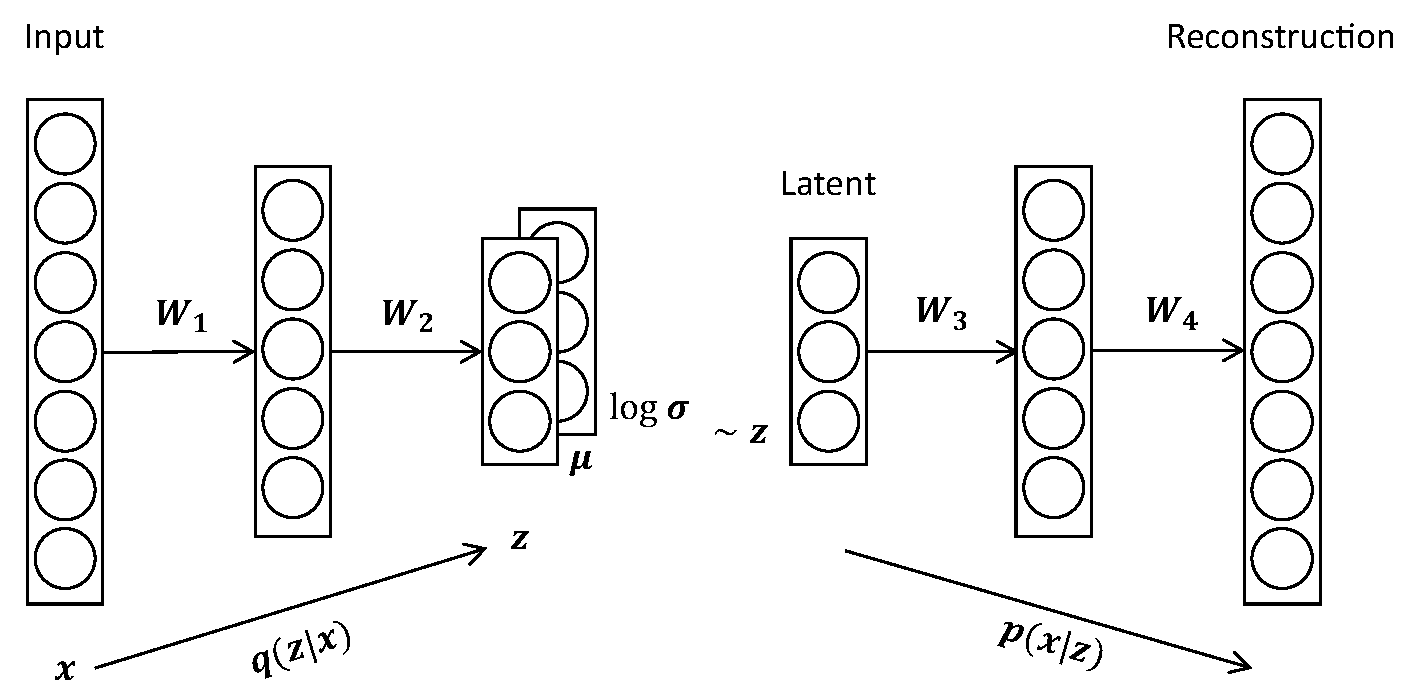
\includegraphics[width=0.5\textwidth]{figures/vae-sample.pdf}
\end{center}
\end{frame}


\begin{frame}{Learned Manifold}
\begin{center}
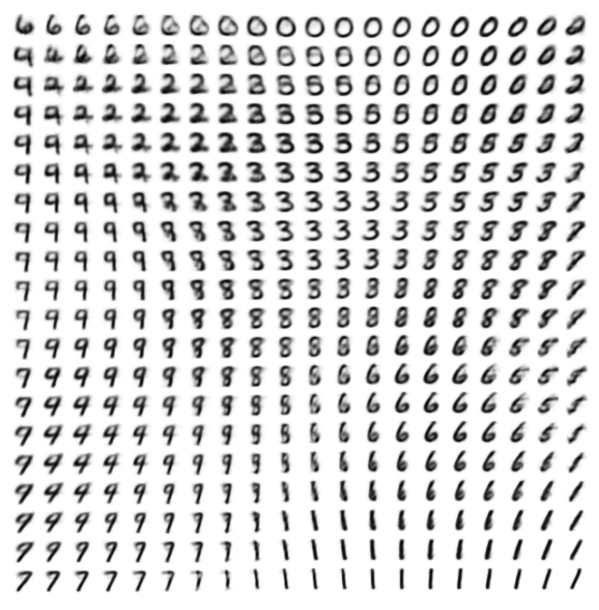
\includegraphics[width=0.45\textwidth]{figures/vae-latent.png}
\end{center}
\end{frame}

% \begin{frame}{Remaining Questions}
% \begin{itemize}
%   \item How to make the latent code correspond to meaningful properties (e.g. shape, color, rotation, size)?
%   \item What if the latent is discrete?
%   \item What if the prior is not Gaussian?
% \end{itemize}
% \end{frame}

% \begin{frame}{Vector Quantization (VQ)}
% \end{frame}

% \begin{frame}{Other Divergence Metrics}
% \end{frame}

% \begin{frame}{Diffusion Models}
% \end{frame}

\begin{frame}{Today's Summary}
\begin{itemize}
  \item<+-> Motivation: Unsupervised learning
  \item<+-> K-means: A simple algorithm for discovering clusters 
  \item<+-> Making k-means probabilistic: Gaussian mixture models
  \item<+-> More generally: Latent variable models
  \item<+-> Learning of latent variable models: EM
  \item<+-> Underlying principle: Maximizing ELBO
  \item<+-> VAE: Introducing variational inference to neural networks. A classic starting example for deep generative modeling.
\end{itemize}
\end{frame}

\section{Conclusion and Outlook}

\begin{frame}{Acknowledgement}
\begin{itemize}
    \item<1-> Most content developed by David Rosenberg (now at Bloomberg).
    \item<1-> Later adapted by He He, Tal Linzen, and others.
    \item<2-> This is a very challenging grad-level course.
    \item<2-> Congrats, you are almost done.
\end{itemize}
\end{frame}

\begin{frame}{Next Lecture: Project Presentation}
\begin{itemize}
    \item Dec 10, in-person presentations.
    \item 22 groups, 120mins.
    \item Aim for \textbf{3 mins} per group, hard stop at 4 mins, and 1 min max for Q\&A.
    \item Send your slides in PDF with your group number by Dec 9 11:59pm (via Google form).
\end{itemize}
\end{frame}

\begin{frame}
{Models}
\begin{description}
\item<1->[Linear] Perceptron, conditional probability models, SVMs
\item<2->[Non-linear] Kernelized models, trees, basis function models, neural nets
\end{description}

\begin{simpleblock}
\onslide<3->{How to choose the model family?}
\begin{itemize}
\onslide<3->{
\item Trade-offs:
\begin{itemize}
\item approximation error and estimation error (bias and variance),
\item accuracy and efficiency (during both training and inference).
\end{itemize}
}
\onslide<4->{
\item Start from the task requirements, e.g. amount of data, computation resource
\item The best lesson is to practice!
}
\end{itemize}
\end{simpleblock}
\note[item]{approximation error and estimation error: high capacity models such as neural nets give you lower approximation error, but the estimation error could be high thus you will need more data compared to other simpler models.}
\note[item]{accuracy and efficiency: you might have time constraints either during training or inference so you might prefer a simpler model even if the accuracy is lower.}
\note[item]{The suggestion is to start from the task requirements and choose your model accordingly.}
\end{frame}

\begin{frame}
{Objectives}
\begin{description}[Loss functions]
\item<1->[Loss functions] How far off a prediction is from the target, e.g. 0-1 loss, margin-based loss, squared loss.
\item<2->[Risk] Expected loss - but expectation over what?
\begin{itemize}
\item<3-> Frequentist approach: expectation over data.
\begin{itemize}
\item Empirical risk minimization, \ie average loss on the training data.
\item Regularization: balance estimation error and generalization error.
\end{itemize}
\item<4-> Bayesian approach: expectation over parameters.
\begin{itemize}
\item Posterior: prior belief updated by observed data.
\item Bayes action minimizes the posterior risk.
\end{itemize}
\end{itemize}
\end{description}
% \note[item]{The next core question in ML is how do we learn the parameters given a model.}
% \note[item]{We covered many loss functions, and you should know when each of them is used.}
% \note[item]{But loss functions depend on the unknown target, thus it's a random variable. We cannot use it to choose model parameters. So we have the notion of risk, or expected loss.}
% \note[item]{If you want a point estimate, you can take the Bayes action which minimizes the posterior risk.}
\end{frame}

\begin{frame}
{Algorithms}
\begin{description}
\item[Learning] Find model parameters---often an optimization problem.
\begin{itemize}
\item (Stocahstic) (sub)gradient descent
\item Functional gradient descent (gradient boosting)
\item Convex vs non-convex objectives
\end{itemize}

\item[Inference] Answer questions given a learned model.
\begin{itemize}
\item Bayesian inference: compute various quantities given the posterior.
\item Dynamic programming: compute $\argmax$ in structured prediction.
\end{itemize}
\end{description}
\note[item]{Given the objective, we still need an algorithm to given us the optimal parameters.}
\note[item]{We refer to finding model params as ``learning'' and it's often an opt problem.}
\note[item]{Another topic we didn't discuss much in this course is inference. Once we find the parameters, how do we use the model to answer questions. For most model we covered, inference is trivial, \eg compute the function values. But there are cases where this can be challenging.}
\end{frame}

\begin{frame}{Do We Still Need ML?}
\begin{itemize}
  \item<+-> Deep Learning (DL) has been overwhelmingly popular in the past few years.
  \item<+-> Many ML methods are considered out-dated.
  \item<+-> However, DL is not necessarily good for all types of data (data availability, data quality, data modality etc.). Classic methods may also have their sweet spots.
  \item<+-> Classic ML sheds new insight into understand DL.
  \item<+-> Classic ML lays down foundation when we innovate in DL algorithms.
\end{itemize}
\end{frame}

\begin{frame}{Other ML Related Advanced Courses in CS/DS}
\begin{itemize}
  {
  \small
    \item Bayesian Machine Learning(Andrew Wilson)
    \item Computer Vision (Saining Xie)
    \item Deep Learning (Yann LeCun)
    \item Deep Reinforcement Learning (Lerrel Pinto)
    \item Embodied Learning and Vision (Mengye Ren)
    \item Foundations of Deep Learning Theory (Matus Telgarsky)
    \item Inference and Representation (Joan Bruna)
    \item Learning with Large Language and Vision Models (Saining Xie)
    \item Mathematics of Deep Learning (Joan Bruna)
    \item Natural Language Processing (He He)
  }
\end{itemize}
\end{frame}

\end{document}
